\documentclass[11pt,fleqn]{exam}
\usepackage[utf8]{inputenc}

\usepackage[margin=1in]{geometry}
\usepackage{amsmath,amssymb}
\usepackage{gensymb}
\usepackage{marvosym}
\usepackage{multicol}
\usepackage{float}
\usepackage{graphicx}
\usepackage{units,icomma}
\usepackage[bahasa]{babel}
\usepackage[colorlinks,linkcolor=blue,urlcolor=blue]{hyperref}
\usepackage[margin=1.5cm]{caption}
\usepackage{wasysym}
\usepackage{tikzsymbols}
\usepackage[shortlabels]{enumitem}
\usepackage{multirow}
\usepackage{fontspec,emoji}

\hyphenation{
  chro-no-ampe-ro-met-ric
  ber-dia-me-ter
  de-ngan
  meng-alam-i
  me-nem-pati
  mic-ro-graphs
  man-hat-tan-henge
  hi-tung-lah}

\addto\extrasbahasa{
	\def\figureautorefname{Gambar}
}

\renewcommand{\figurename}{Gambar.}
\def\equationautorefname{Persamaan}
\newcommand{\class}{OLIMPIADE ASTRONOMI}
\newcommand{\term}{Tingkat Nasional - 2023 (Teori)}
\newcommand{\examnum}{OSN Astronomi 2023}
%\newcommand{\examdate}{11/02/2014}
%\newcommand{\timelimit}{120 Minutes}

%%%%%%%%% Units and Symbols
\newcommand*{\kms}{km s\ensuremath{^{-1}}}
\newcommand*{\Msun}{\ensuremath{M_{\odot}}}
\newcommand*{\Lsun}{\ensuremath{L_{\odot}}}
\newcommand*{\Rsun}{\ensuremath{R_{\odot}}}
\newcommand*{\Mstar}{\ensuremath{M_{\star}}}
\newcommand*{\Lstar}{\ensuremath{L_{\star}}}
\newcommand*{\Rstar}{\ensuremath{R_{\star}}}

\newcommand*{\jam}{\ensuremath{^{j}}}
\newcommand*{\h}{\ensuremath{^{h}}}
\newcommand*{\m}{\ensuremath{^{m}}}
\newcommand*{\s}{\ensuremath{^{s}}}
\newcommand*{\de}{\ensuremath{^{\circ}}}
\newcommand*{\am}{'}
\newcommand*{\as}{''}

\newcommand*{\alp}{\ensuremath{\alpha}}
\newcommand*{\del}{\ensuremath{\delta}}


\pagestyle{head}
\firstpageheader{}{}{}
\runningheader{\examnum}{}{Halaman \thepage\ dari \numpages}
\runningheadrule


\begin{document}

\noindent
\begin{tabular*}{\textwidth}{l @{\extracolsep{\fill}} r @{\extracolsep{6pt}} l}
\textbf{\class} \\% & \textbf{Name:} & \makebox[2in]{\hrulefill}\\
\textbf{\term}  %&&\\
%\textbf{\examnum} &&\\
%\textbf{\examdate} &&\\
%\textbf{Time Limit: \timelimit} & Teaching Assistant & \makebox[2in]{\hrulefill}
\end{tabular*}\\
\rule[2ex]{\textwidth}{2pt}

\noindent
\begin{tabular}{ll}
Copyright (c) 2023 & Ridlo W. Wibowo (ridloww@gmail.com)\\
                   & Sulistiyowati (lis.sulistiyowt@gmail.com)
\end{tabular}

\vspace{0.3cm}
\noindent
Solusi ini dibuat tanpa jaminan kesesuaian dengan solusi resmi dari juri olimpiade sains bidang Astronomi. Pengguna boleh menyebarluaskan dan/atau memodifikasi solusi ini dengan mencantumkan sumber asli. Hak cipta soal ada pada Kemendiknas dan dilindungi undang-undang. Jika ada kesalahan jawaban/penulisan harap melaporkan ke alamat surel di atas.

\vspace{0.4cm}
\noindent
\rule[2ex]{\textwidth}{1.5pt}

% \textbf{Soal Pilihan Ganda}
\bigskip
\begin{questions}

\question Supernova Tycho, pada tahun 1572, mencapai kecerlangan maksimum yakni -4 magnitudo pada tanggal 1 Oktober, dan sejak itu mengalami peredupan hingga akhirnya tidak tampak oleh mata tanpa alat bantu pada 1 Maret 1574. Jika kecerlangan semu $b$ pada saat $t$ setelah 1 Oktober 1572 berkaitan dengan kecerlangan semu $b_0$ melalui persamaan
\begin{equation*}
    b = b_0 10^{-t/\tau}
\end{equation*}
maka
\begin{enumerate}[a.]
    \item tentukanlah nilai $\tau$ (sertakan satuannya)
    \item tentukanlah tanggal terakhir seorang pengamat masih dapat mengamati supernova tersebut jika menggunakan teleskop berdiameter 150 mm.
\end{enumerate}


\newpage
\textit{Jawaban:}
\begin{enumerate}[a.]
    \item Persamaan yang diberikan menggambarkan perubahan kecerlangan supernova secara eksponensial menurun, dengan nilai $b_0$ adalah nilai kecerlangan saat $t=0$ yaitu pada tanggal 1 Oktober 1572. Untuk mencari nilai $\tau$, dapat kita gunakan pernyataan bahwa supernova tersebut tidak tampak oleh mata telanjang pada 1 Maret 1574, yang artinya magnitudo supernova saat itu adalah 6 mag. 

    Karena tidak ada detail satuan waktu, maka kita bebas menggunakan satuan waktu apa saja untuk parameter $t$, paling mudah tentu dalam satuan hari (begitu juga untuk $\tau$). Jika kita nyatakan dalam satuan hari, maka nilai $t$ saat 1 Maret 1574 dihitung sejak 1 Oktober 1572 adalah 516 hari.
    \begin{eqnarray*}
        m - m_0 &=& -2,5 \log{\frac{b}{b_0}}\\
        6 + 4 &=& -2,5 \log{\left( 10^{-t/\tau} \right)}\\
        -4 &=& -\frac{t}{\tau}\\
        \tau &=& \frac{t}{4} = \frac{516}{4}\\
        \tau &=& 129 \text{ hari}
    \end{eqnarray*}

    \item Kemampuan teleskop mengumpulkan cahaya akan sebanding dengan luas bukaan teleskop atau sebanding juga dengan diameter kuadrat, $\propto D^2$. Pada kasus ini kita diminta untuk mencari limit batas terlihatnya supernova, sehingga semakin besar diameter, ``batas fluks'' yang dapat teramati akan menjadi lebih kecil, yang artinya malah berbanding terbalik dengan diameter kuadrat. Kita \textbf{asumsikan} diameter pupil mata saat gelap sekitar 7 mm.
    \begin{eqnarray*}
        \frac{b_\text{limit telekop}}{b_\text{limit mata}} &=& \left(\frac{D_\text{mata}}{D_\text{teleskop}}\right)^2\\ 
        \frac{b_0 10^{-\frac{t_\text{tele}}{\tau}}}{b_0 10^{-\frac{t_\text{mata}}{\tau}}} &=& \left( \frac{7}{150} \right)^2\\
        10^{\frac{t_\text{mata} - t_\text{tele}}{\tau}} &=& \left( \frac{7}{150} \right)^2\\
        \frac{t_\text{mata} - t_\text{tele}}{\tau} &=& \log{\left(\left(\frac{7}{150}\right)^2\right)}\\
        516 - t_\text{tele} &=& 129 \cdot 2 \cdot \log{\frac{7}{150}}\\
        t_\text{tele} &=& 859,4 \text{ hari} \rightarrow 860 \text{ hari} \quad \text{sejak 1 Oktober 1572}
    \end{eqnarray*}
    Sehingga dapat disimpulkan bahwa tanggal terakhir supernova dapat diamati menggunakan teleskop 150 mm adalah 8 Februari 1575*. \\
    
    *Catatan: tidak melewati tahun kabisat dan belum melewati transisi Julian ke Gregorian pada 4 Oktober 1582.
\end{enumerate}


\newpage
\question Sebuah satelit buatan berada pada orbit MEO (\textit{Medium Earth Orbit}) pada ketinggian 2000 km dari permukaan Bumi. Orbit satelit dianggap berbentuk lingkaran dengan periode orbit adalah 2 jam. Anggap pula Bumi berbentuk bola sempurna dengan jejari 6378 km. Misalkan stasiun pengendali satelit berada di Kabupaten Rote Ndao pulau Rote (provinsi Nusa Tenggara Timur) di lintang $11^\circ$ LS, $123^\circ$ BT. Bidang orbit satelit ini diketahui memiliki kemiringan sebesar $11^\circ$ terhadap ekuator Bumi.
\begin{enumerate}[a.]
    \item Hitunglah kecepatan sudut orbit satelit ini dinyatakan dalam satuan radian jam$^{-1}$.
    \item Hitung pula kecepatan linear orbit satelit ini dinyatakan dalam satuan km jam$^{-1}$.
    \item Buatlah satu gambar sketsa dengan setidaknya dua komponen gambar: lingkaran orbit satelit dan lingkaran di permukaan Bumi yang melewati stasiun tersebut.
    \item Dengan mengabaikan faktor rotasi Bumi, hitung berapa lama satelit ini dapat terlihat di atas horison lokasi stasiun pengendali! Nyatakan hingga satuan detik dan bulatkan tanpa pecahan.
    \item Dengan anggapan yang sama seperti soal 2d, hitung pula berapa lama satelit ini dapat terlihat di atas horison suatu wilayah di Indonesia di lintang 0$^\circ$ LS, 123$^\circ$ BT! Nyatakan hingga satuan detik dan dibulatkan tanpa pecahan.
\end{enumerate}


\newpage
\textit{Jawaban:}

Dapat dibuktikan bahwa nilai ketinggian dan periode satelit sebetulnya tidak terlalu cocok dengan massa Bumi seharusnya. Jika kita anggap kedua nilai benar, maka massa Bumi menjadi $6,7 \times 10^{24}$ kg, sedikit lebih besar dari seharusnya. Walaupun demikian untuk menjawab soal-soal berikutnya kita bisa anggap kedua nilai sudah benar! :)
\begin{enumerate}[a.]
    \item Kecepatan sudut orbit satelit dapat dihitung dari periode,
    \begin{eqnarray*}
        \omega &=& \frac{2 \pi}{T}\\
        \omega &=& \frac{2 \pi}{2} = \pi = 3,1415926... \text{ rad/jam}
    \end{eqnarray*}
    
    \item Kecepatan linier orbit satelit,
    \begin{eqnarray*}
        v &=& \omega \cdot r\\
        v &=& \pi \cdot 8378 = 26320,26 \text{ km/jam}
    \end{eqnarray*}

    \item Asumsikan saat satelit di titik paling Selatan bertepatan dengan bujur pengamat, sehingga pengamat dapat melihatnya di zenit (kemiringan orbit sama dengan lintang pengamat). Jika demikian, kita bisa gambarkan masalah ini seperti berikut,
    \begin{figure}[!ht]
        \centering
        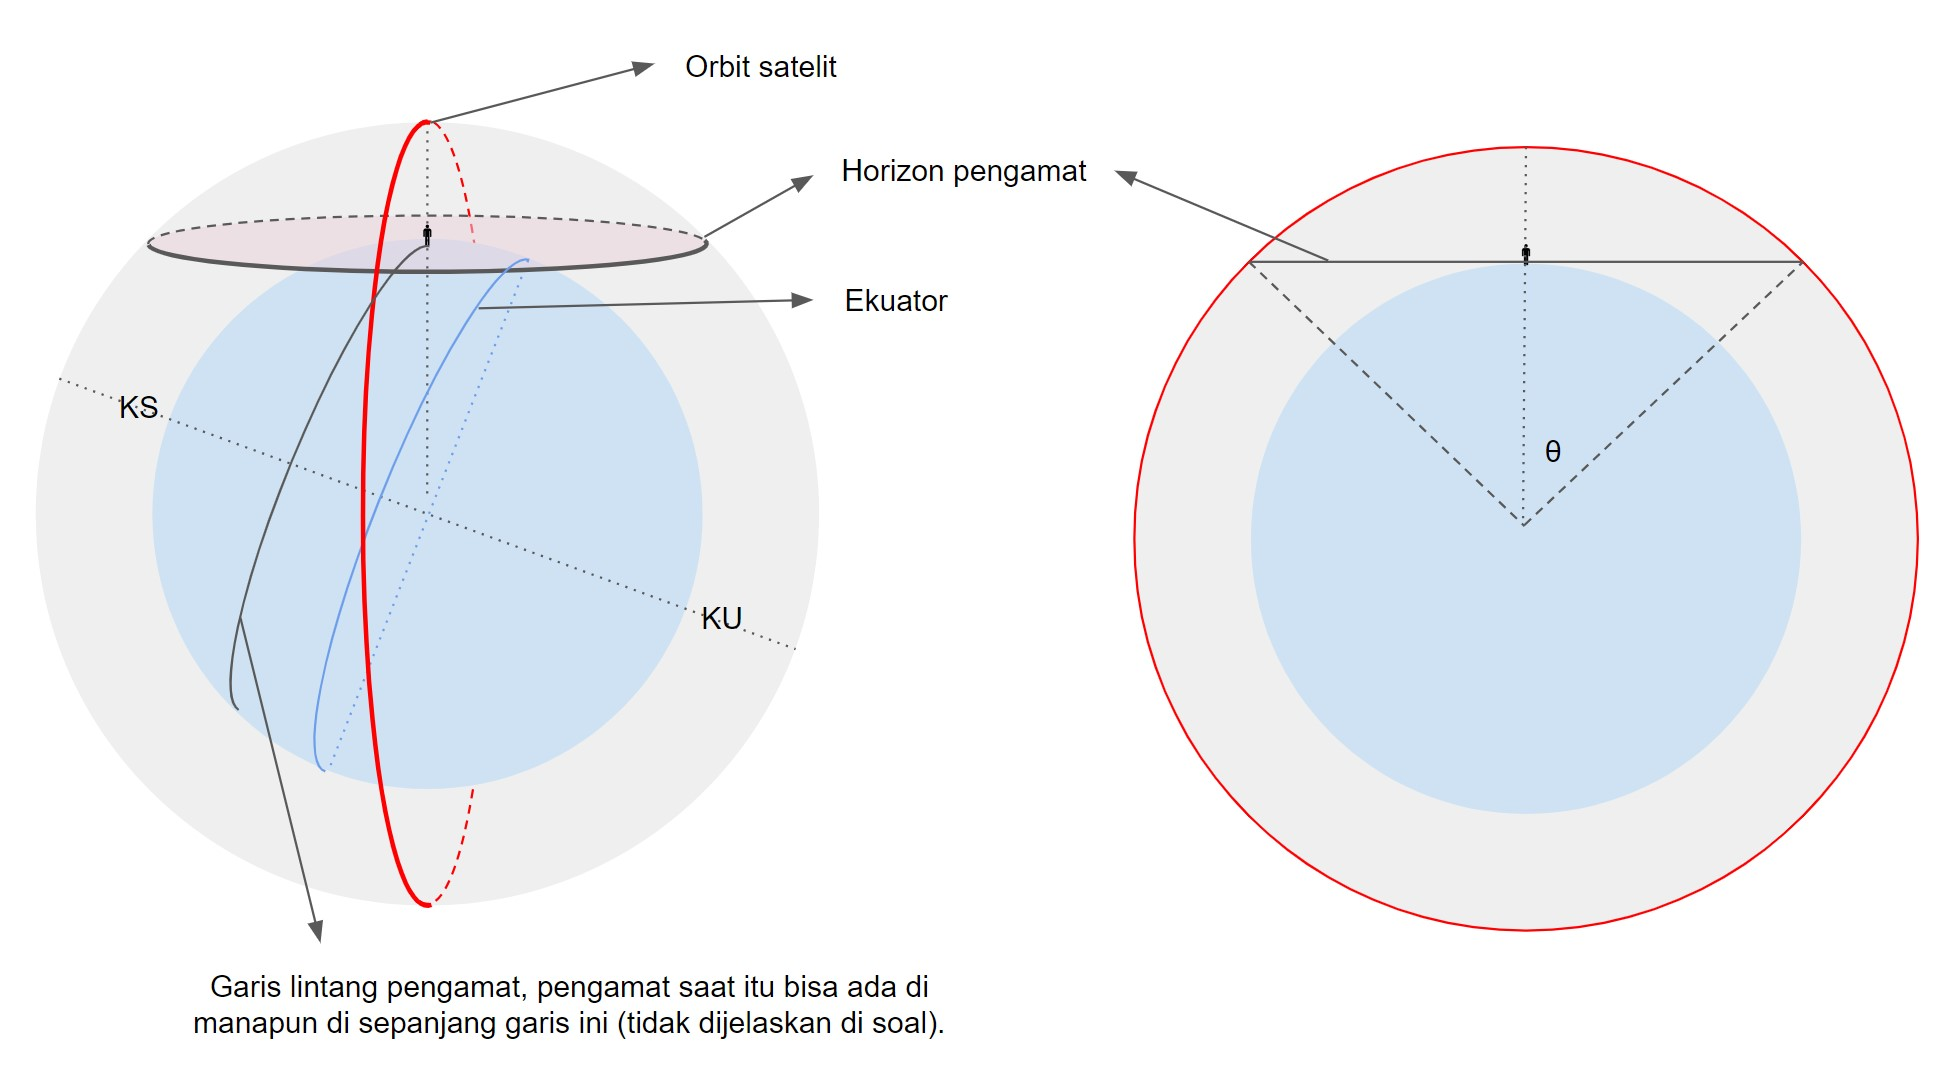
\includegraphics[width=0.9\textwidth]{osn2023_2_kasus1.jpg}
    \end{figure}

    \item Dengan asumsi posisi relatif pengamat di atas, serta mengabaikan rotasi Bumi (karena satelit berjalan cepat), maka untuk menghitung lama satelit di atas horizon pengamat dapat dilakukan dengan mencari $\theta$,
    \begin{eqnarray*}
        \cos{\theta} &=& \frac{R_{\oplus}}{R_\oplus + h}\\
        \cos{\theta} &=& \frac{6378}{6378 + 2000}\\
        \theta &=& 40,42287033177^{\circ}\\
        \Delta t &=& \frac{2 \theta}{360^{\circ}} \cdot T = \frac{2 \cdot 40,42287033177^{\circ}}{360^{\circ}} \cdot 2^\text{h}  = 0,44914300369^{\text{h}} = 26^{\text{m}} 57^{\text{s}}  
    \end{eqnarray*}

    \item Pada soal ini tidak diberikan lagi posisi relatif orbit satelit (titik nodal) terhadap pengamat di ekuator. Kita asumsikan mirip dengan soal sebelumnya satelit berada di titik paling Selatan saat melewati bujur pengamat,
    \begin{figure}
        \centering
        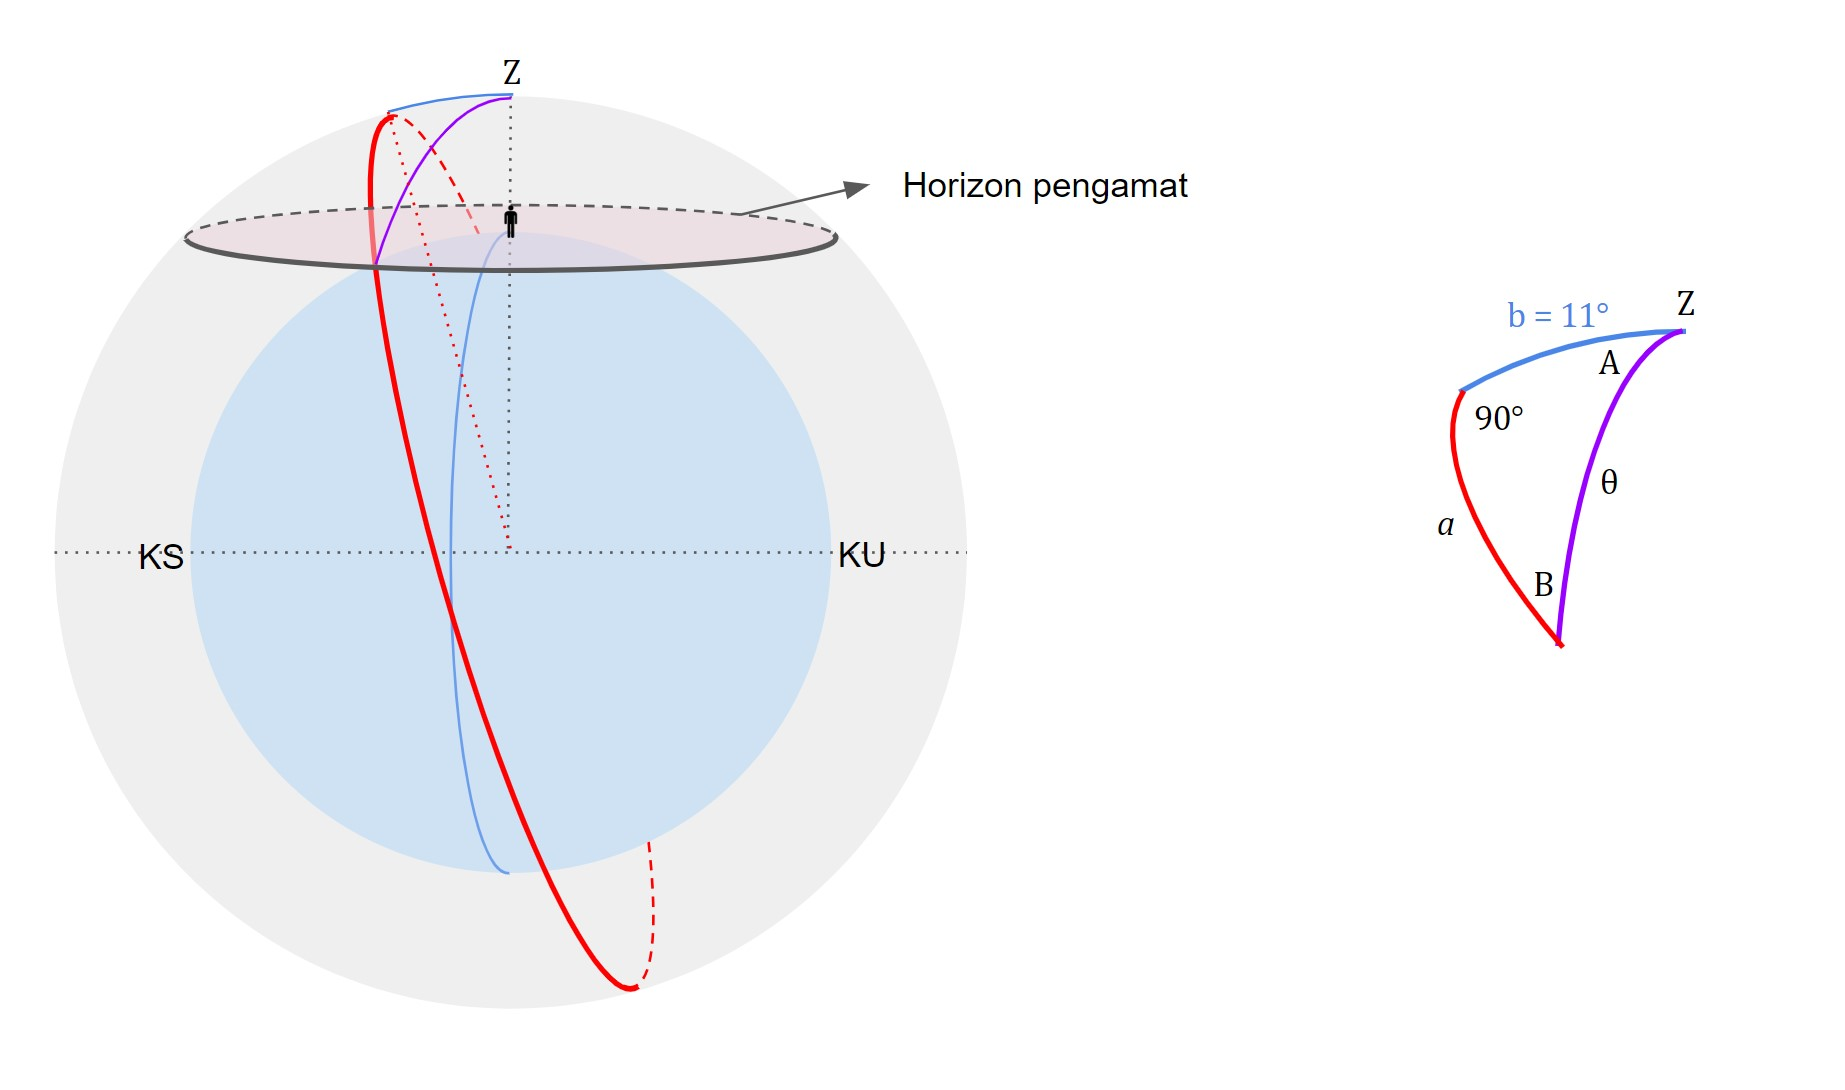
\includegraphics[width=0.8\textwidth]{osn2023_2_kasus2.jpg}
    \end{figure}

    Untuk mencari lamanya satelit di atas horizon, kita dapat menghitung nilai $a$,
    \begin{eqnarray*}
        \cos{\theta} &=& \cos{a} \cos{b} + \sin{a} \sin{b} \cos{90^\circ}\\
        \cos{\theta} &=& \cos{a} \cos{b}\\
        \cos{a}  &=& \frac{\cos{(40,42287033177^{\circ})}}{\cos{(11^\circ})}\\
        a &=& 39,14705636^\circ\\
        \Delta t &=& \frac{2 a}{360^{\circ}} \cdot T = 26^\text{m} 6^\text{s}
    \end{eqnarray*}

    Waktu yang dihitung ini adalah waktu terpendek satelit di atas horizon pengamat di ekuator. Waktu terpanjangnya sama dengan soal sebelumnya, yaitu ketika zenit pengamat bertepatan dengan titik nodal orbit satelit.
    
    Kuis tambahan \emoji{fire} \emoji{fire}: 
    \begin{itemize}
        \item Hitung azimut satelit saat terbit dan terbenam!
        \item Untuk kasus soal 2d, hitung perbandingan kecepatan sudut saat di horizon dengan saat di zenit!
    \end{itemize}
\end{enumerate}


\newpage
\question Diketahui data massa dan luminositas untuk bintang-bintang yang sedang berada di fase evolusi Deret Utama berikut ini:
\begin{table}[!h]
    \centering
    \begin{tabular}{|c|c|}
    \hline
    $M/M_\odot$ & $L/L_\odot$ \\
    \hline
          0,10 & 0,003 \\
     \hline
          0,50 & 0,03 \\
     \hline
          0,75 & 0,3 \\
     \hline
          1,0 & 1 \\
     \hline
          1,5 & 5 \\
     \hline
          3,0 & 60 \\
     \hline
          5,0 & 600 \\
     \hline
          10 & 10000 \\
     \hline
          15 & 17000 \\
     \hline
          25 & 80000 \\
     \hline
          60 & 790000 \\
     \hline
    \end{tabular}
    \label{tab:tabel_no3}
\end{table}
\begin{enumerate}[a.]
    \item Dari data tersebut buatlah plot luminositas sebagai fungsi dari massa dalam skala logaritmik.
    
    \item Dari grafik di soal 3a, buatlah persamaan garis dari titik-titik data dalam bentuk $y=ax + b$, dengan $a$ dan $b$ untuk setiap baris data ke-$i$ memenuhi hubungan:
    \begin{eqnarray*}
        a &=& \frac{n \left(\Sigma x_i y_i \right) - \left(\Sigma x_i \right)\left(\Sigma y_i \right)}{n\Sigma x_i^2 - \left(\Sigma x_i \right)^2}\\
        b &=&\frac{ \left(\Sigma y_i \right)\left(\Sigma x_i^2 \right) - \left(\Sigma x_i \right) \left(\Sigma x_i y_i \right)}{n\Sigma x_i^2 - \left(\Sigma x_i \right)^2}
    \end{eqnarray*}
    dengan $n$ menunjukkan jumlah data. Cantumkan juga nilai-nilai yang diperlukan dalam perhitungan $a$ dan $b$.

    \item Diketahui sebuah bintang mempunyai luminositas $55L_\odot$ dan temperatur efektif 8000 K. Dari persamaan garis di soal 3b, tentukanlah massa (dalam $M_\odot$) dan kemudian tentukan radius bintang (dalam $R_\odot$).

    \item Hitunglah total energi bintang di soal 3c, dengan mengasumsikan kerapatan di dalam bintang konstan, menggunakan persamaan energi potensial gravitasi:
    \begin{equation*}
        E_\text{gr} = - \frac{3}{5} \frac{GM^2}{R}
    \end{equation*}
    (tanda negatif - menunjukkan gaya tarik gravitasi materi di dalam bintang membuat bintang tersebut dalam keadaan stabil).

    \item Hitunglah usia bintang di soal 3c (nyatakan dalam satuan tahun)
\end{enumerate}


\newpage
\textit{Jawaban:}
\begin{enumerate}[a.]
    \item Untuk dapat membuat plot data (soal a) dan regresi linier (soal b) sebaiknya kita buat tabel tambahan terlebih dahulu, hal ini juga diminta untuk dicantumkan pada soal b.
    \begin{table}[!h]
    \centering
    \begin{tabular}{|c|c|c|c|c|c|}
    \hline
    $M/M_\odot$ & $L/L_\odot$ & $x_i$ & $y_i$ & $x_i^2$ & $x_i y_i$ \\
    & & $\left[\log{(M/M_\odot)} \right]$ & $\left[\log{(L/L_\odot)}\right]$ & &\\
    \hline
    0,1 & 0,003 & -1,000 & -2,523 & 1,000 & 2,523\\ 
    \hline
    0,5 & 0,03 & -0,301 & -1,523 & 0,091 & 0,458\\ 
    \hline
    0,75 & 0,3 & -0,125 & -0,523 & 0,016 & 0,065\\ 
    \hline
    1 & 1 & 0,000 & 0,000 & 0,000 & 0,000\\ 
    \hline
    1,5 & 5 & 0,176 & 0,699 & 0,031 & 0,123\\ 
    \hline
    3 & 60 & 0,477 & 1,778 & 0,228 & 0,848\\ 
    \hline
    5 & 600 & 0,699 & 2,778 & 0,489 & 1,942\\ 
    \hline
    10 & 10000 & 1,000 & 4,000 & 1,000 & 4,000\\ 
    \hline
    15 & 17000 & 1,176 & 4,230 & 1,383 & 4,975\\ 
    \hline
    25 & 80000 & 1,398 & 4,903 & 1,954 & 6,854\\ 
    \hline
    60 & 790000 & 1,778 & 5,898 & 3,162 & 10,487\\ 
    \hline
    \hline
     \multicolumn{2}{|c|}{$n = 11$}  & $\Sigma x_i = 5,278$ & $\Sigma y_i  = 19,718$ & $\Sigma x_i^2 = 9,353$ & $\Sigma x_i y_i = 32,276$\\
    \hline
    \end{tabular}
    \label{tab:tabel_no3}
    \end{table}

    \begin{figure}[!h]
        \centering
        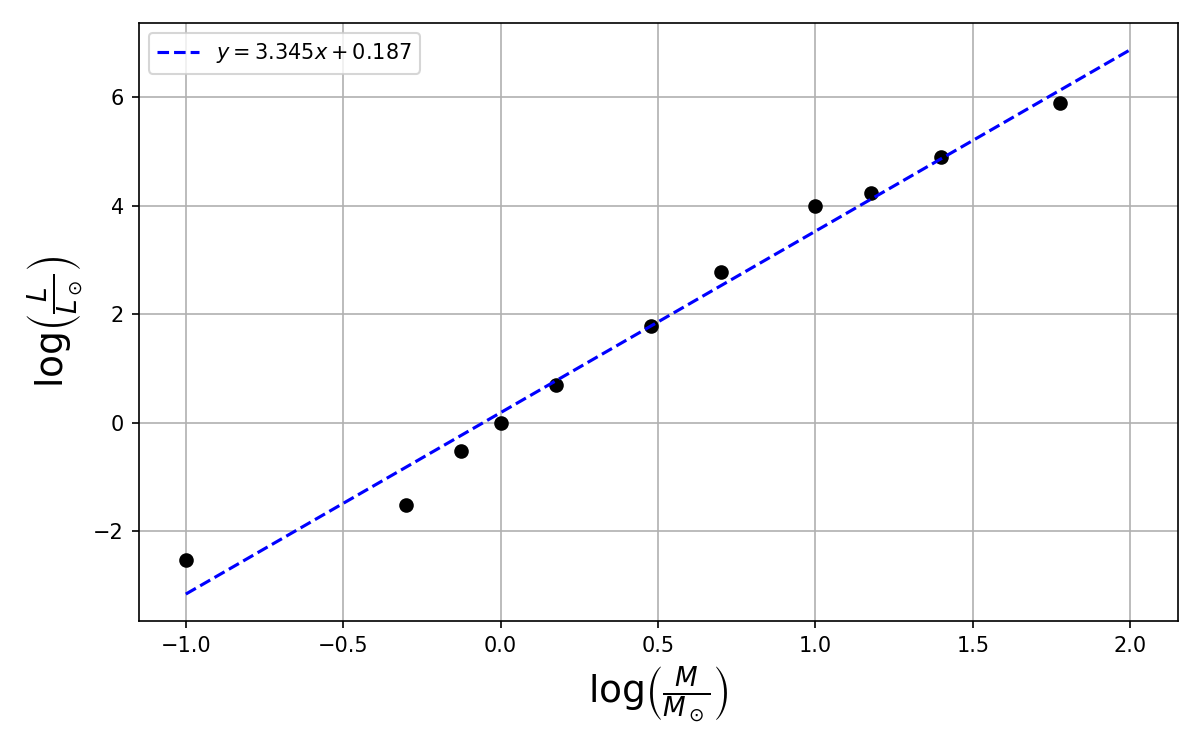
\includegraphics[width=0.8\textwidth]{osn_no3.png}
        %\caption*{Hasil plot data.}
        \label{fig:osn3}
    \end{figure}

    \item Menggunakan nilai-nilai hasil perhitungan yang ada di tabel, maka hasil regresinya sebagai berikut:
    \begin{equation*}
        a  = \frac{11 \cdot 32,276 - 5,278 \cdot 19,718}{11 \cdot 9,353 - 5,278^2} = 3,345
    \end{equation*}
    
    \begin{equation*}
        b = \frac{19,718 \cdot 9,353 - 5,278 \cdot 32,276}{11 \cdot 9,353 - 5,278^2} = 0,187
    \end{equation*}

    Persamaan hasil regresi 
    \begin{equation*}
    \log{\left( \frac{L}{L_\odot} \right)} = 3,345 \cdot \log{\left( \frac{M}{M_\odot} \right)} + 0,187  
    \end{equation*}
    atau kita juga bisa ubah dalam bentuk pangkat,
    \begin{equation*}
         \frac{L}{L_\odot}  = 1,54 \left( \frac{M}{M_\odot} \right)^{3,345}
    \end{equation*}

    \item Kita dapat menggunakan persamaan hasil regresi untuk memperkirakan massa bintang,
    \begin{eqnarray*}
        M &=& 10^{\frac{\log{(55)} - 0,187}{3,345}}\\
        M &=& 2,91 M_\odot
    \end{eqnarray*}
    Radius bintang dapat dicari dengan data temperatur dan luminositas yang telah diberikan. Kita bisa gunakan suhu Matahari sekitar 5772 K (bisa juga 5800 atau 6000 K tergantung hafalan).
    \begin{eqnarray*}
        \frac{L}{L_\odot} &=& \frac{4 \pi R^2 \sigma T^4}{4 \pi R_{\odot}^2 \sigma T_{\odot}^4}\\
        \frac{L}{L_\odot} &=& \left( \frac{R}{R_\odot} \right)^2 \left( \frac{T}{T_\odot} \right)^4\\
        55 &=& \left( \frac{R}{R_\odot} \right)^2 \left( \frac{8000}{5772} \right)^4\\ 
        R &=& 3,86 R_\odot 
    \end{eqnarray*}
    Jika nilai temperatur Matahari yang digunakan berbeda maka hasilnya akan sedikit berbeda ($3,86-4,17 R_\odot$). 
    
    \item Energi potensial gravitasi yang terkandung di dalam bola dengan kerapatan seragam (\textit{uniform}) dengan radius $R$ diberikan di soal,
    \begin{equation*}
        U = - \frac{3}{5} \frac{GM^2}{R}
    \end{equation*}
    Andaikan sebuah bintang mengerut dari awan dengan radius sangat besar ($R \approx \infty$), maka perubahan energi potensial selama proses pengerutan adalah
    \begin{eqnarray*}
        \Delta U &=& U_\text{akhir} - U_\text{awal}\\
        \Delta U &=& - \frac{3}{5} \frac{GM^2}{R} - 0\\
        \Delta U &=& - \frac{3}{5} \frac{GM^2}{R}
    \end{eqnarray*}
    tanda minus artinya bahwa energi potensial gravitasi menurun selama proses pengerutan. 
    
    Total perubahan energi potensial yang terjadi adalah
    \begin{eqnarray*}
        \Delta U &=& \frac{3}{5} \frac{G (2,91 M_\odot)^2}{3,86 R_\odot}\\
        \Delta U &=& 5 \times 10^{41} \text{ Joule}
    \end{eqnarray*} 
    Catatan: Kami menggunakan nilai hafalan untuk massa dan radius Matahari: $M_\odot = 2\times 10^{30}$ kg, dan $R_\odot = 696000$ km.

    \item Berdasarkan hukum kekekalan energi dan teorema virial yang bekerja pada sistem gravitasi, kita bisa memperkirakan bahwa ketika awan molekular / protobintang mengalami pengerutan dengan penurunan energi potensial gravitasi sebesar $\Delta U$, maka hal ini akan disertai dengan peningkatan energi kinetik partikel-partikel di dalam awan sebesar $\frac{1}{2} \Delta U$ dan $\frac{1}{2} \Delta U$ sisanya akan diradiasikan.
    \begin{eqnarray*}
        E_\text{tersedia untuk diradiasikan}  = \frac{1}{2} \Delta U = \frac{3}{10} \frac{GM^2}{R}
    \end{eqnarray*}
    Energi tersebut akan dipancarkan selama proses pengerutan secara perlahan. Andaikan selama proses pengerutan energi yang dipancarkan tetap sebesar $L$, maka lama waktu yang dibutuhkan adalah
    \begin{equation*}
        t_{KH} = \frac{\frac{3}{10} \frac{GM^2}{R}}{L} 
    \end{equation*}
    Sebuah perkiraan/skala kasar tentang berapa lama suatu proses di bintang terjadi yang disebut dengan skala waktu termal atau skala waktu Kelvin-Helmholtz. 

    Usia bintang pada soal 3c yang ditanyakan menurut skala waktu termal, yakni perkiraan kasar lama waktu yang dibutuhkan untuk berubah dari awan protobintang menjadi bintang Deret Utama adalah
    \begin{equation*}
        t = \frac{0,5 \cdot 5 \times 10^{41}}{55 \cdot 3,86 \times 10^{26}} = 1,187 \times 10^{13} \text{ detik} = 376075 \text{ tahun}
    \end{equation*}

   *Catatan: pertanyaan ``usia bintang'' diberikan setelah pada soal sebelumnya diberitahu mengenai rumus ``total energi potensial'' yang dimiliki bintang, seolah mengarahkan peserta untuk menghitung skala waktu termal. Asumsi kami sepertinya pembuat soal ingin memberitahukan bahwa bintang pada soal 3c adalah bintang Deret Utama yang \textit{baru saja lahir} dan peserta diminta menghitung lama ia ``dikandungan''. :)
\end{enumerate}


\newpage
\question Di dalam mekanika benda langit, gaya sentral dapat diartikan secara sederhana sebagai gaya yang mengarah ke pusat lingkaran. Tinjau dua benda bermassa $M$ dan $m$. Jika sistem dua benda ini digambarkan melalui sistem koordinat bola ($r, \theta, \phi$), maka gaya sentral adalah gaya yang dialami oleh benda $m$ akibat kehadiran medan gaya karena keberadaan benda $M$ yang arahnya menuju pusat benda $M$, yang secara matematis ditulis $F_c = f(r)$, dengan kata lain gaya hanya merupakan fungsi dari koordinat jarak $r$. Hukum kuadrat kebalikan merupakan kasus khusus dari gaya sentral, yakni ketika $f(r) = \frac{k}{r^2}$, dengan $k$ = konstanta. Untuk memudahkan pembahasan, kita terapkan persoalan ini pada kasus planet mengitari Matahari dengan orbit lingkaran sempurna. Planet dengan massa $m_p$ mengitari Matahari dengan massa $M_\odot$ dengan jejari orbit $R$.

Aturan penyelesaian soal ini:

Dalam bentuk apapun \underline{tidak diperbolehkan} menggunakan
\begin{itemize}
    \item Hukum Gravitasi Newton
    \item Hukum III Kepler
\end{itemize}

\begin{enumerate}[a.]
    \item Dengan menggunakan ungkapan gaya sentral dan unsur-unsur (rumus-rumus) kinematika rotasi, tunjukkan bahwa 
    \begin{equation*}
        \frac{P^2}{R^3} = C
    \end{equation*}
    dengan $P$ dan $C$ secara berurutan menyatakan periode dan sebuah konstanta. Kemudian tuliskan bentuk eksplisit dari konstanta $C$. Tuliskan dengan jelas hukum-hukum dan asumsi-asumsi yang digunakan di setiap tahap penyelesaian.
\end{enumerate}
Butir-butir soal di bawah ini ($b$, $c$, $d$, dan $e$) bertujuan untuk memperoleh bentuk eksplisit dari konstanta $k$ yang muncul pada $F_c = \frac{k}{R^2}$
\begin{enumerate}[a.]\setcounter{enumi}{1}
    \item Tunjukkan secara analitis menggunakan argumen-argumen hukum gerak Newton bahwa selain terdapat hubungan $k \propto m_p$, juga terdapat hubungan $k \propto M_\odot$.
    \item Telah ditunjukkan bahwa $k$ bergantung pada massa planet dan massa Matahari. Di bawah ini diberikan dua bentuk hubungan $k$ dengan $m_p$ dan $M_\odot$. Periksalah kemasukakalan dari hubungan-hubungan tersebut, simpulkan hubungan mana yang benar, dan mengapa bukan yang lainnya?
    \begin{enumerate}[i.]
        \item $k \propto m_p + M_\odot$
        \item $k \propto m_p M_\odot$
    \end{enumerate}
    \item Apakah hubungan $k \propto m_p(m_p + M_\odot)$ juga benar? Jelaskan!
    \item Tuliskan secara eksplisit (lengkap) bentuk gaya sentral $F_c$ sebagai fungsi dari $m_p$, $M_\odot$, dan $R$, sesuai dengan jawaban-jawabanmu pada butir-butir sebelumnya, dan turunkan pula dimensi dari konstanta kesebandingannya, lalu berikan tanggapan atas hal tersebut.
\end{enumerate}


\newpage
\textit{Jawaban:}
\begin{enumerate}[a.]
    \item Jika kita asumsikan Matahari diam, lalu planet bergerak melingkari Matahari, maka berdasarkan kinematika rotasi, seharusnya yang berperan sebagai gaya sentripetal yang menahan planet untuk tidak lepas (gerak lurus) adalah gaya sentral,
    \begin{eqnarray*}
        F_\text{sentripetal} &=& F_\text{sentral}\\
        m_p a_\text{sentripetal} &=& F_g(R)\\
        m_p \frac{v^2}{R} &=& F_g(R)\\
        m_p\frac{4 \pi^2 R^2}{P^2 R} &=& F_g(R)\\
        m_p\frac{4 \pi^2 R}{P^2} &=& F_g(R)\\
        \frac{P^2}{R} F_g(R) &=& m_p 4 \pi^2
    \end{eqnarray*}
    Untuk bisa \textit{memenuhi} Hukum Kepler yang telah ditemukan sebelumnya, 
    \begin{equation*}
        \frac{P^2}{R^3} = C = \text{konstan}
    \end{equation*}
    maka pastilah gaya sentral $F_g(R)$ harus berbanding terbalik dengan $R^2$, atau kita bisa tuliskan $F_g(R) = \frac{k}{R^2}$, dengan $k$ adalah suatu konstanta, sehingga,
    \begin{eqnarray*}
        \frac{P^2}{R} \cdot \frac{k}{R^2} &=& m_p 4 \pi^2\\
        \frac{P^2}{R^3} &=& \frac{m_p 4 \pi^2}{k}
    \end{eqnarray*}
    Kita peroleh konstanta yang dimaksud soal $C = \frac{m_p 4 \pi^2}{k}$
    
    \item Berdasarkan hukum gerak Newton yang kedua ($\sum \textbf{F} = m \textbf{a}$), maka gaya gravitasi akan sebanding dengan massa dan percepatan gravitasi ($a_g$)
    \begin{eqnarray*}
        F_g = m a_g
    \end{eqnarray*}
    dari pengukuran diketahui bahwa percepatan benda yang jatuh di permukaan Bumi \textit{tidak bergantung} pada massa benda tersebut, sehingga bisa disimpulkan bahwa 
    \begin{eqnarray*}
        F_g \propto m
    \end{eqnarray*}
    kemudian dengan menggunakan hukum gerak Newton yang ketiga, aksi = reaksi ($\textbf{F}_{12} = -\textbf{F}_{21}$), maka seharusnya gaya gravitasi akan sebanding juga dengan massa benda lainnya, $M$
    \begin{eqnarray*}
        F_g \propto M    
    \end{eqnarray*}

    \item Berdasarkan argumen hukum gerak Newton yang kedua yang telah dituliskan di atas, jika gaya gravitasi sebanding dengan $k \propto m + M$, maka percepatan gravitasi yang dirasakan suatu benda akan menjadi
    \begin{eqnarray*}
        m a &=& \frac{\text{konstanta} \cdot (m + M)}{R^2}\\
        a &=& \frac{\text{konstanta}}{R^2} \frac{(m + M)}{m}\\
        a &=& \frac{\text{konstanta}}{R^2} \left(1 + \frac{M}{m}\right)\\
    \end{eqnarray*}
    Andaikan kita terapkan pada kasus di permukaan Bumi dengan $M$ adalah massa Bumi dan $m$ adalah benda yang jatuh dipercepat di permukaan Bumi, maka menggunakan rumus di atas akan terjadi hal yang \textit{tidak masuk akal}, benda yang massanya lebih kecil akan mengalami percepatan lebih besar dibanding benda yang bermassa besar. Pensil yang jatuh akan mengalami percepatan lebih besar dibanding mobil yang jatuh di permukaan Bumi.

    Hubungan yang lebih tepat adalah $k \propto m \cdot M$, percepatan suatu benda akan sesuai dengan massa benda yang lain. Benda yang jatuh di permukaan Bumi akan memiliki percepatan yang sama, yang bergantung massa Bumi (bukan massa benda yang jatuh), hal ini sesuai dengan fakta pengamatan.
    
    \item Jika kita terapkan gaya gravitasi sebanding dengan $m_p (m_p + M_\odot)$, maka hal ini tidak akan memenuhi hukum gerak Newton yang ketiga. Berdasarkan hukum gerak ketiga Newton, gaya gravitasi yang diakibatkan planet terhadap Matahari harus sama besar dengan gaya gravitasi yang diakibatkan Matahari terhadap planet. Jika menggunakan keproporsionalan di soal, maka sudah jelas besar gaya gravitasi akan berbeda jika kita tuliskan untuk planet, $\propto m_p (m_p + M_\odot)$, dengan apabila kita tuliskan untuk Matahari $\propto M_\odot (m_p + M_\odot)$
    
    \item Dapat disimpulkan bahwa gaya sentral yang dapat mendeskripsikan gaya gravitasi harusnya akan berbentuk
    \begin{eqnarray*}
        F_g &\propto& \frac{m_p M_\odot}{R^2}\\ 
        F_g &=& \text{konstanta} \frac{m_p M_\odot}{R^2}
    \end{eqnarray*}

    Konstanta pada persamaan gaya gravitasi yang diturunkan akan memiliki satuan,
    
    N m$^2$ kg$^{-2}$ = kg m s$^{-2}$ $\cdot$ m$^2$ kg$^{-2}$ = kg m$^{3}$ s$^{-2}$ 
    
    Dimensi konstanta: $ML^{3}T^{-2}$

    Tanggapan: Capek bang... 
\end{enumerate}




\newpage
\question \begin{enumerate}[a.]
    \item \textbf{Bagian I}
    \begin{enumerate}[i.]
        \item Secara teori, pada gugus galaksi, galaksi-galaksi dalam daerah yang sudah berada dalam keadaan setimbang \textit{virial} mengikuti kaidah teorema \textit{virial}: $2 E_\text{kinetik} + E_\text{potensial} = 0$. Radius pada daerah setimbang \textit{virial} ini disebut radius \textit{virial}. Kemudian didefinisikan massa total gugus sebagai penjumlahan dari seluruh massa masing-masing galaksi
        \begin{equation*}
            M = \sum_i m_i
        \end{equation*}
        dispersi kecepatan yang diberi bobot massa
        \begin{eqnarray*}
            \left< v^2 \right> = \frac{1}{M} \sum_i m_i v_i^2
        \end{eqnarray*}
        dan radius gravitasi
        \begin{equation*}
            r_G = 2M^2 \left( \sum_{i \neq j} \frac{m_i m_j}{r_{ij}} \right)^{-1}
        \end{equation*}
        dengan $r_{ij}$ = jarak spasial/ruang antara galaksi $i$ dan galaksi $j$. Tuliskan rumus estimasi massa gugus dengan menerapkan teorema virial! 

        \item Karena jarak spasial $r_{ij}$ yang merupakan jarak 3-dimensi tidak dapat diukur secara langsung, maka dilakukan perubahan dari jarak spasial menjadi jarak terproyeksi di bidang langit antara galaksi $i$ dan galaksi $j$. Hubungan radius gravitasi terproyeksi $(R_G)$ dengan jarak terproyeksi $(R_{ij})$ adalah
        \begin{equation*}
            R_G = 2M^2 \left( \sum_{i \neq j} \frac{m_i m_j}{R_{ij}} \right)^{-1}
        \end{equation*}
        Untuk kasus distribusi kecepatan isotropik (atau distribusi kecepatan simetri bola) berlaku relasi $\left< v^2 \right> = 3 \sigma_v^2$ dan $r_G = \frac{\pi}{2} R_G$. Parameter $\sigma_v$ dan $R_G$ didapatkan dari pengamatan. Tinjau gugus galaksi Abell yang diamati secara optis. Apabila didapatkan $\sigma_v = 900 \text{ km s}^{-1}$ dan $R_G = 1,4$ Mpc, berapakah massa gugus tersebut dalam satuan massa Matahari ($M_\odot$)?
    \end{enumerate}
    
    \item \textbf{Bagian II}
    \begin{enumerate}[i.]
        \item Berdasarkan pengamatan pada panjang gelombang sinar-X, untuk daerah kesetimbangan virial berlaku hubungan temperatur dan massa gugus, $T \propto \frac{M}{r}$. Gugus galaksi diasumsikan berbentuk bola. Hubungan temperatur sebagai fungsi dari massa saja dituliskan sebagai $T \propto M^{\alpha}$. Berapakah nilai $\alpha$?

        \newpage
        \item Kemudian dari observasi gugus-gugus galaksi didapatkan grafik berikut:
        
        \begin{figure}[!ht]
            \centering
            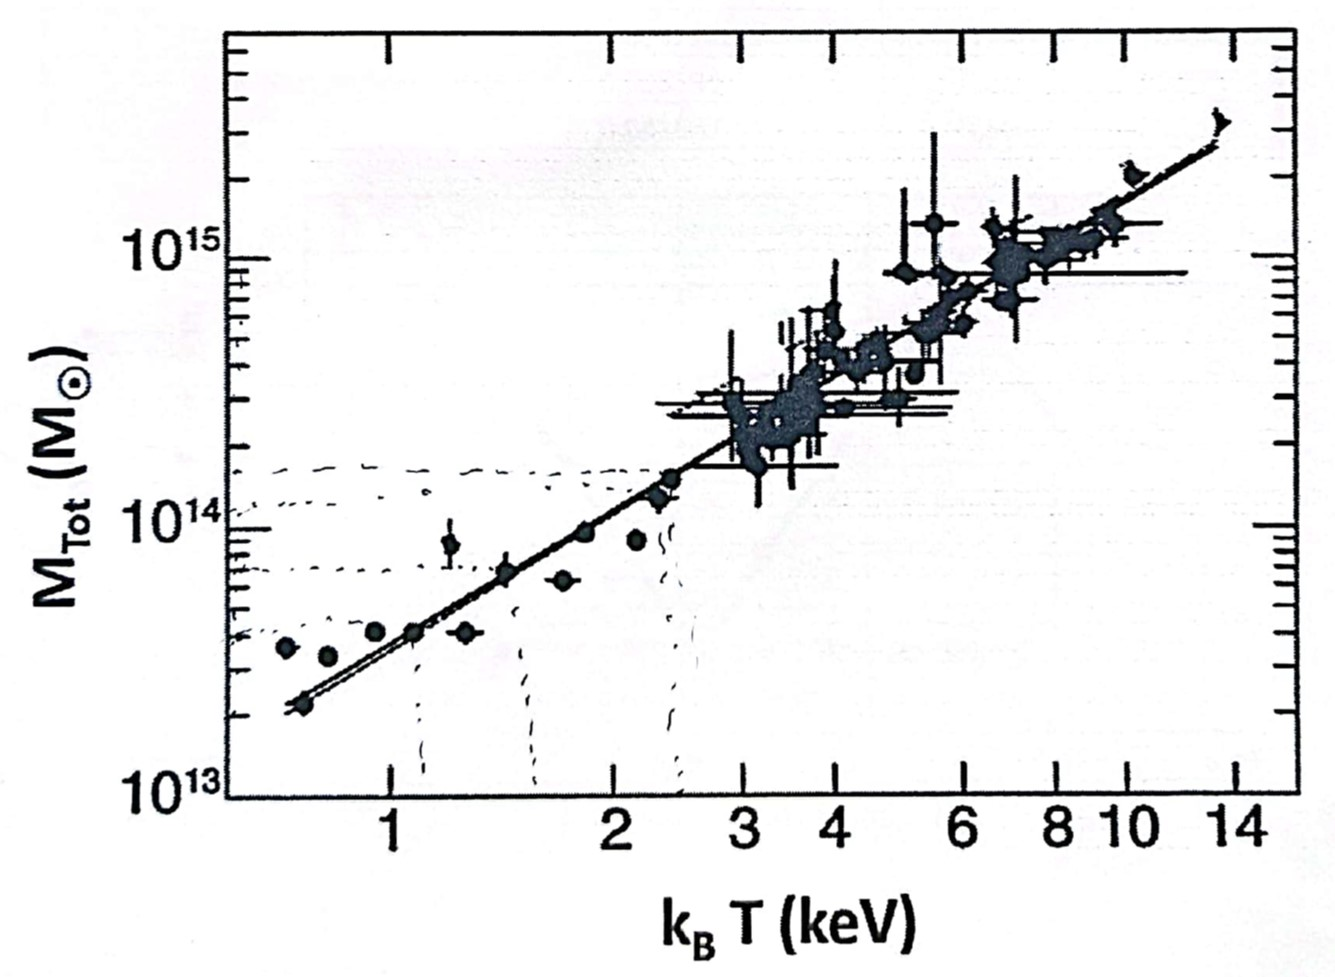
\includegraphics[width=0.6\textwidth]{osn_soal5.jpg}
            %\caption{Caption}
            %\label{fig:enter-label}
        \end{figure}
        
        Dari grafik di atas, tuliskan rumus massa gugus sebagai fungsi dari temperatur (dalam hal ini satuan rumus massa adalah $M_\odot$)! Apakah rumus ini konsisten dengan soal b (Bagian II) butir $i$? Jelaskan!

        \item Untuk massa gugus sebesar $1 \times 10^{14} M_\odot$, berapakah temperatur gugus?
    \end{enumerate}
\end{enumerate}


\newpage
\textit{Jawaban:}

\begin{enumerate}[a.]
    \item Bagian I
    \begin{enumerate}[i]
        \item Total energi kinetik sistem:
        $$T = \sum_{i=1}^n \frac{1}{2}  m_i v_i^2$$
        Total energi potensial sistem:
        $$U = \frac{1}{2} \sum_{i=1, i \neq j}^n \frac{G m_i m_j}{r_{ij}}$$
        Faktor $\frac{1}{2}$ pada energi potensial supaya tiap ``pasang'' benda/massa tidak terhitung dua kali energi potensialnya, karena  fungsi \texttt{sum}/$\Sigma$ di atas indeks $i$ dan $j$ mengulang untuk benda yang sama.
        
        Selanjutnya menggunakan teorema virial,
        \begin{eqnarray*}
            2 T &=& U\\
            2 \cdot \frac{1}{2} \sum_i m_i v_i^2 &=& \frac{1}{2} G \sum_{i \neq j} \frac{m_i m_j}{r_{ij}}\\
            M \left< v^2 \right> &=& G \frac{M^2}{r_G}\\
            M &=& \frac{r_G \left< v^2 \right>}{G}
        \end{eqnarray*}

        \item Pada kenyataannya nilai kecepatan tiap galaksi $v_i$ pada ruang 3D tidak dapat diperoleh dengan mudah. Hanya kecepatan radial ($v_r$) yang langsung bisa diperoleh dari pengamatan efek Doppler. Dengan asumsi isotropik / simetri bola dan hubungan $v_{ri} = v_i \cos{\theta_i}$ dengan $\theta_i$ adalah sudut antara arah garis pandang ke galaksi $i$ dengan arah vektor kecepatan galaksi tersebut terhadap pusat massa sistem, kita bisa turunkan bahwa 
        $$\left< v^2 \right> = \sigma^2_{v_{tot}} = 3 \sigma_{v_{r}}^2$$
        Di sisi lain, jarak antar galaksi $r_{ij}$ juga sulit untuk diperoleh, yang mudah untuk diukur adalah jarak terproyeksinya di langit ($R_{ij}$). Keduanya memiliki hubungan $R_{ij} = r_{ij} \sin{\xi_{ij}}$ dengan $\xi_{ij}$ adalah sudut antara arah garis pandang ke galaksi $i$ dengan vektor posisi yang mengarah dari galaksi $i$ ke galaksi $j$. Kemudian bisa diturunkan faktor koreksi yang menghubungkan total energi potensial yang seharusnya dihitung menggunakan jarak sebenarnya dengan apabila menggunakan jarak terproyeksi, hal ini kemudian akan menghasilkan
        $$r_G = \frac{\pi}{2} R_G \quad \text{dengan} \quad R_G = 2M^2 \left( \sum_{i \neq j} \frac{m_i m_j}{R_{ij}} \right)^{-1}$$
        Jika dispersi kecepatan radial dan jarak terproyeksi antar galaksi kita peroleh, maka massa gugus galaksi dapat kita estimasi
        \begin{eqnarray*}
            M &=& \frac{r_G \left< v^2 \right>}{G} \\
            M &=& \frac{\frac{\pi}{2} R_G \cdot 3 \sigma_{v_r}^2}{G}
        \end{eqnarray*}
        Untuk nilai $\sigma_{v_r} = 900$ kms$^{-1}$ dan $R_G = 1,4$ Mpc, akan kita peroleh massa gugus galaksi sebesar $M = 2,47 \times 10^{45}$ kg = $1,236 \times 10^{15} M_\odot$.
    \end{enumerate}
    
    \item Bagian II
    \begin{enumerate}[i.]
        \item Pada soal diberikan hubungan,
        \begin{eqnarray*}
            T_\text{vir} \propto \frac{M_\text{vir}}{r_\text{vir}}
        \end{eqnarray*}
        sedangkan asumsi simetri bola memberikan hubungan
        \begin{eqnarray*}
            M_\text{vir} &=& \frac{4}{3} \pi r_\text{vir}^3 \bar{\rho}\\
            r_\text{vir} &=& \left(\frac{3 M_\text{vir}}{4 \pi \bar{\rho}}\right)^{\frac{1}{3}} \text{ atau}\\
            r_\text{vir} &\propto& M_\text{vir}^{\frac{1}{3}}
        \end{eqnarray*}
        sehingga dapat disimpulkan,
        \begin{equation*}
            T_\text{vir} \propto M^{\frac{2}{3}}
        \end{equation*}  
        Jadi nilai $\alpha = \frac{2}{3}$.

        \item Plot yang diberikan dalam skala logaritmik dengan basis 10, termasuk untuk sumbu-$x$ (silakan buktikan!).  
        \begin{figure}[!ht]
            \centering
            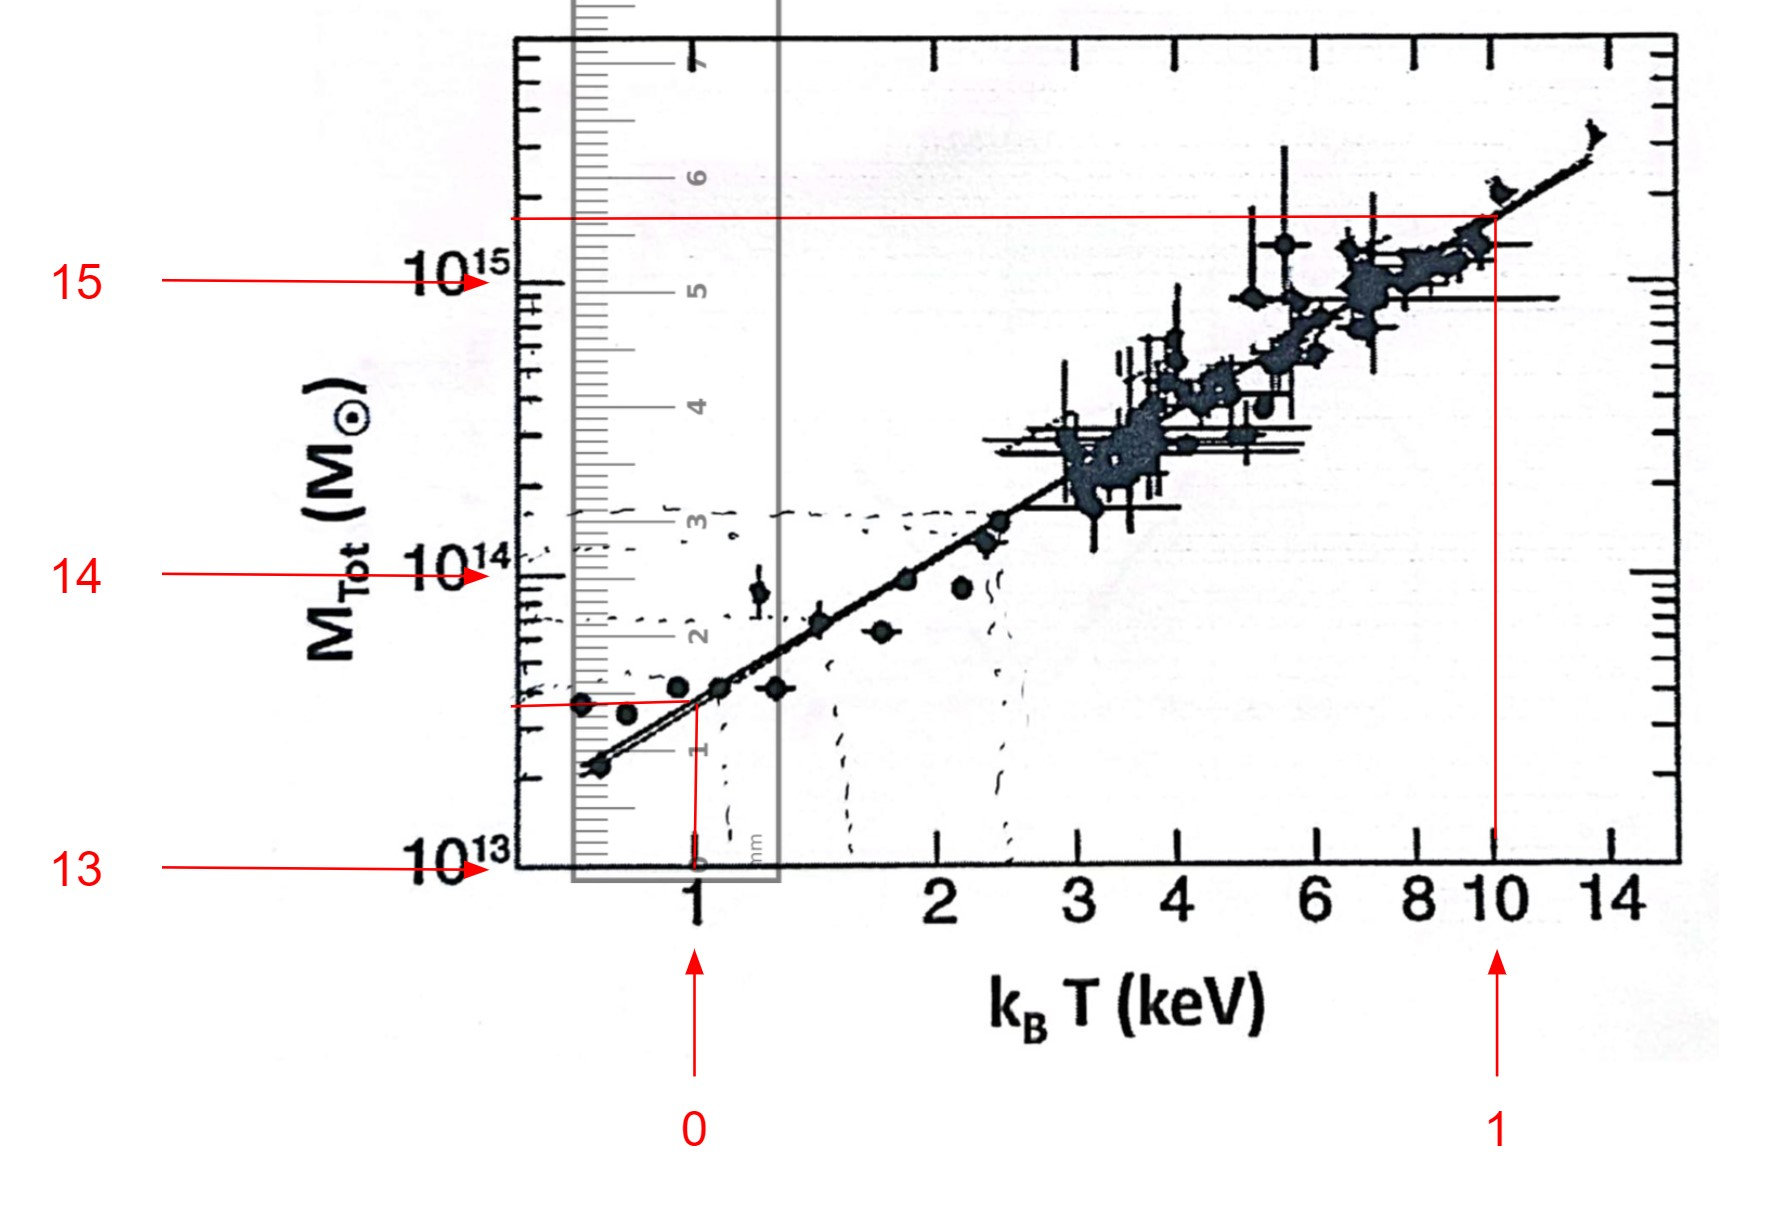
\includegraphics[width=0.9\textwidth]{osn_jwb5.jpg}
        \end{figure}

        Kita ambil 2 titik sampel untuk mencari persamaan garis hasil \textit{fitting}. Untuk nilai yang kita pilih, misalnya $x_1 = 0$ dan $x_2 = 1$ kita cari nilai $y$ yang sesuai dengan bantuan penggaris.
        \begin{eqnarray*}
            y_1 &=& 13 + \frac{14 \text{ mm}}{25,5 \text{ mm}} = 13,54901961 \quad (M_\text{Tot} = 3,54 \times 10^{13} M_\odot)\\
            y_2 &=& 13 + \frac{56,5 \text{ mm}}{25,5 \text{ mm}} = 15,21568627 \quad (M_\text{Tot} = 1,643 \times 10^{15} M_\odot)
        \end{eqnarray*}

        Persamaan garis dapat diturunkan dari kesebangunan segitiga,
        \begin{eqnarray*}
            \frac{y - y_1}{y_2 - y_1} &=& \frac{x - x_1}{x_2 - x_1}\\
            \frac{y - 13,54901961}{15,21568627 - 13,54901961} &=& \frac{x - 0}{1 - 0}\\
            y &=& 1,6666667 x + 13,54901961
        \end{eqnarray*}
        Karena $y = \log_{10}{\frac{M_\text{Tot}}{M_\odot}}$ dan $x = \log_{10}{\frac{k_B T}{1 \text{ keV}}}$, maka dapat dituliskan 
        \begin{eqnarray*}
            \log_{10}{\left(\frac{M_\text{Tot}}{M_\odot}\right)} &=& 1,6666667\log_{10}{\left(\frac{k_B T}{1 \text{ keV}}\right)} + 13,54901961
        \end{eqnarray*}
        dapat juga diturunkan persamaan dalam bentuk pangkat,
        \begin{eqnarray*}
            \log_{10}{\left(\frac{M_\text{Tot}}{M_\odot}\right)} &=& \log_{10}{\left(\left(\frac{k_B T}{1 \text{ keV}}\right)^{1,6666667}\right)} + \log_{10}{\left(10^{13,54901961}\right)}\\
            \log_{10}{\left(\frac{M_\text{Tot}}{M_\odot}\right)} &=& \log_{10}{\left(\left(\frac{k_B T}{1 \text{ keV}}\right)^{5/3} \cdot 10^{13,54901961}\right)}\\
            \frac{M_\text{Tot}}{M_\odot} &=& 3,54 \times 10^{13} \left(\frac{k_B T}{1 \text{ keV}}\right)^{5/3}
        \end{eqnarray*}
        Hasil \textit{fitting} data menunjukkan bahwa $M \propto T^{5/3}$ atau $T \propto M^{3/5}$, dapat disimpulkan bahwa nilai $\alpha = 3/5$ yang diperoleh sedikit lebih kecil dari hasil teori ``sederhana'' pada butir soal Bagian II (i) yang menunjukkan nilai $\alpha = 2/3$.

        \item Temperatur gugus bisa dicari dari persamaan bentuk log atau bentuk pangkat. Kita gunakan bentuk log karena lebih mudah
        \begin{eqnarray*}
            \left( \frac{k_B T}{1 \text{ keV}} \right) &=& \frac{14 - 13,54901961}{5/3}\\
            k_B T &=& 0,270588 \text{ keV} = 270,6 \text{ eV} \qquad \text{[energi ini dalam rentang \textit{soft x-ray}]} \\
            T &=& 3,14 \text{ juta Kelvin}. 
        \end{eqnarray*}
        
    \end{enumerate}
\end{enumerate}


\newpage
\question Sebuah sistem bintang ganda sinar-\textit{X} yang terdiri dari bintang neutron dan sebuah bintang redup, beredar dengan orbit lingkaran mengelilingi titik pusat massa sistem. Pengamatan spektroskopi menghasilkan data kecepatan radial pada tabel dan grafik sebagai berikut,

\begin{table}[!h]
    \centering
    \begin{tabular}{|c|c|c|c|}
    \hline
    Waktu pengamatan & Waktu pengamatan & \multicolumn{2}{|c|}{Kecepatan Radial}\\
    \cline{3-4}
    (\textit{Julian Day} atau JD)& ($\text{JD}-2460186,25$) & $v_1$ (km s$^{-1}$) & $v_2$ (km s$^{-1}$)\\
    \hline
    2460186,250000 & 0,000000 & -5,50 & 393,50\\
    \hline
    2460186,253472 & 0,003472 & -8,25 & 590,25\\
    \hline
    2460186,256944 & 0,006944 & -11,00 & 787,00\\
    \hline
    2460186,260417 & 0,010417 & -8,25 & 590,25\\
    \hline
    2460186,263889 & 0,013889 & -5,50 & 393,50\\
    \hline
    2460186,267361 & 0,017361 & -2,75 & 196,75\\
    \hline
    2460186,270833 & 0,020833 & 0,00 & 0,00\\
    \hline
    2460186,274306 & 0,024306 & -2,75 & 196,75\\
    \hline
    2460186,277778 & 0,027778 & -5,50 & 393,50\\
    \hline
    2460186,281250 & 0,031250 & -8,25 & 590,25\\
    \hline
    2460186,284722 & 0,034722 & -11,00 & 787,00\\
    \hline
    2460186,288194 & 0,038194 & -8,25 & 590,25\\
    \hline
    2460186,291667 & 0,041667 & -5,50 & 393,50\\
    \hline
    \end{tabular}
    % \caption{Caption}
    % \label{tab:my_label}
\end{table}

\begin{figure}[!ht]
    \centering
    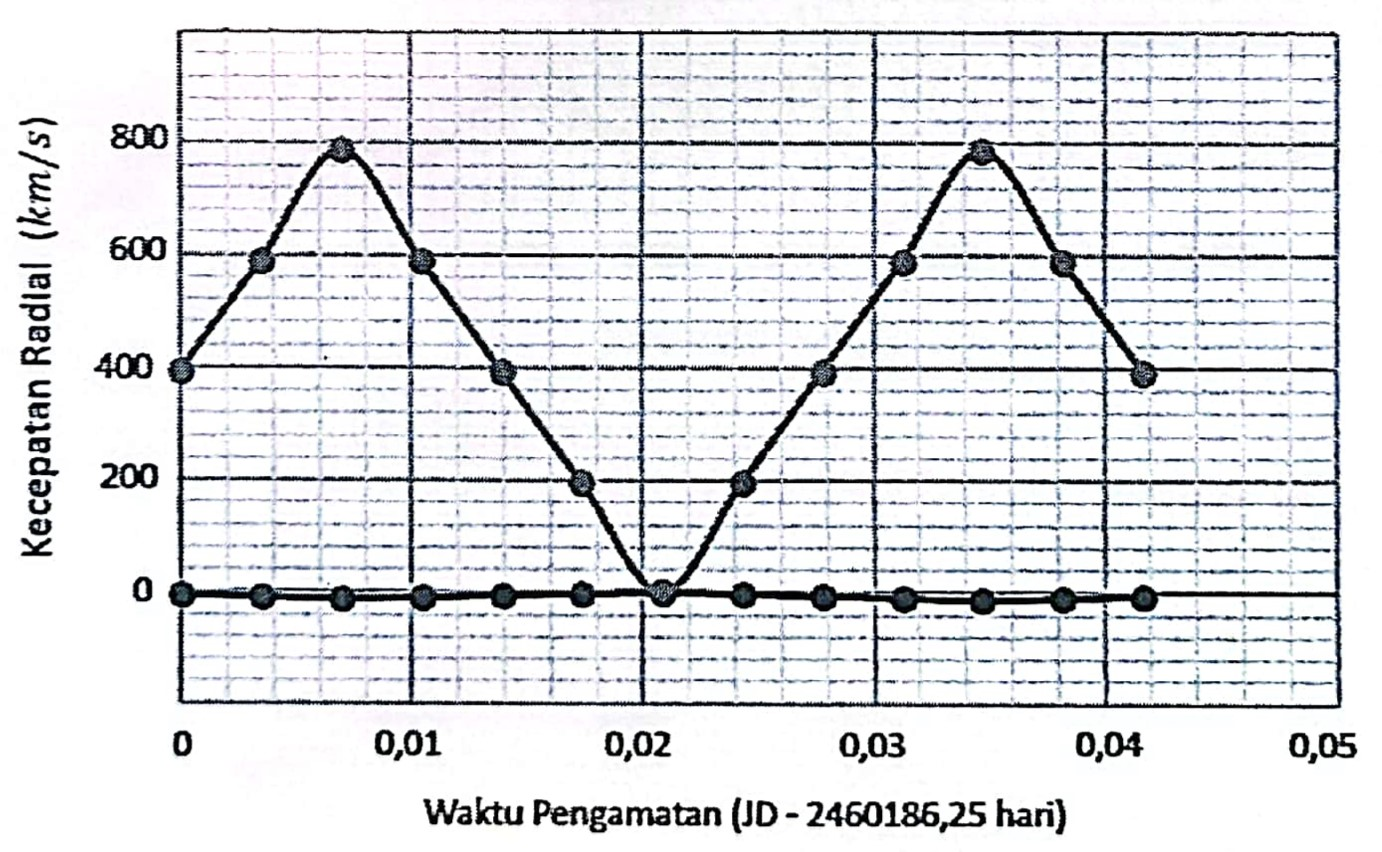
\includegraphics[width=0.75\textwidth]{soal_no6.jpg}
    %\caption{Caption}
    %\label{fig:enter-label}
\end{figure}

Hitunglah
\begin{enumerate}[a.]
    \item radius orbit bintang neutron (dalam satuan km),
    \item radius orbit bintang redup (dalam satuan km),
    \item massa total kedua bintang (nyatakan dalam satuan massa Matahari),
    \item massa bintang redup (dalam satuan massa Matahari).
\end{enumerate}


\newpage
\textit{Jawaban:}

Data kurva kecepatan radial yang diberikan bertolak belakang dengan pernyataan bahwa mereka adalah suatu sistem bintang ganda yang saling mengorbit pusat massa. Jika memang mereka adalah satu sistem bintang ganda, maka sudah seharusnya `tengah' atau rata-rata dari kurva kecepatan radial masing-masing bintang akan berhimpit dan merupakan kecepatan radial sistem. Pada data dan plot yang diberikan, hal tersebut tidak ditemukan, bintang satu ($v_1$) konsisten bergerak mendekati kita sedangkan bintang dua ($v_2$) selalu menjauhi kita, yang artinya mereka bergerak saling menjauh satu sama lain. Selain itu tidak diberikan juga data inklinasi orbit.

\vspace{1cm}
\textbf{Jika datanya benar} dan disederhanakan sebagai kasus dengan inklinasi orbit 90$^\circ$, kita bisa lakukan tahapan dasar berikut ini:
\begin{enumerate}[i.]
    \item cari periode ($P$) dari plot, misal dari melihat waktu yang dibutuhkan dari puncak ke puncak
    \item menggunakan amplitudo kecepatan radial, $(v_{r,\text{max}} - v_{r,\text{min}})/2$, sebagai kecepatan orbit masing-masing bintang ($v_1$ dan $v_2$). Jika tidak diketahui inlinasi, maka kecepatan radial tersebut adalah $v_r = v \sin{i}$.
    \item menghitung radius orbit masing-masing bintang $r_1 = \frac{v_1 P}{2 \pi}$, $r_2 = \frac{v_2 P}{2 \pi}$.
    \item semimayor orbit $a = r_1 + r_2$
    \item massa total sistem dari hukum III Kepler, $\frac{a^3}{P^2} = (m_1 + m_2)$
    \item massa masing-masing bintang dari massa total dan hubungan pusat massa $\frac{m_1}{m_2} = \frac{v_2}{v_1} = \frac{r_2}{r_1}$.
\end{enumerate}

\vspace{1cm}
Kita berbaik sangka saja, mungkin kami yang belum paham atau memang soal ini untuk menguji pemahaman siswa, karena terlalu mudah \emoji{joy} \emoji{leaves}...

\newpage
\question \textit{Planetary nebula} (PN) merupakan bagian dari evolusi lanjut bintang bermassa rendah atau menengah. PN terdiri dari sebuah bintang pusat yang diselubungi oleh gas dan debu yang berasal dari angin bintang. Berikut ini merupakan data spektrum dan magnitudo yang teramati dari PN.

\begin{figure}[ht!]
    \centering
    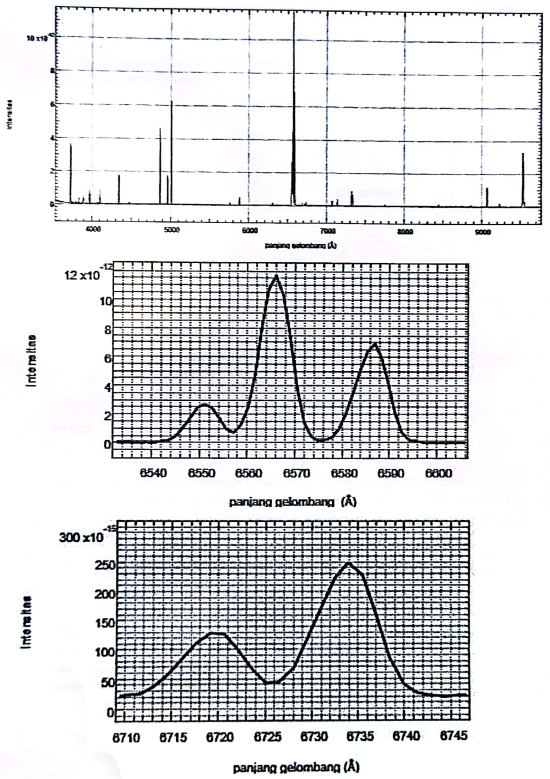
\includegraphics[scale=0.7]{PN.png}
    % \caption{Caption}
    % \label{fig:enter-label}
\end{figure}

\begin{table}[!ht]
\centering
% \caption{Comparison of percentages.}
\begin{tabular}{|c|c|}
\hline
\multicolumn{2}{|c|}{Magnitudo}\\ 
\hline
U   & 13,196\\
\hline
B   & 13,158\\
\hline
V   & 12,831\\
\hline
\end{tabular}
\end{table}

\begin{enumerate}[a.]
    \item Berdasarkan informasi garis emisi dari deret Balmer (H$\alpha$), tentukan kecepatan radial PN dalam km s$^{-1}$. Diketahui konstanta Rydberg $R=10970910$ m$^{-1}$.
    \item Diketahui garis sulfur terionisasi dapat digunakan untuk menentukan kerapatan elektron di selubung PN. Dengan bantuan plot berikut dan spektrum PN, tentukanlah kerapatan elektron di selubung PN.

    \begin{figure}[ht!]
        \centering
        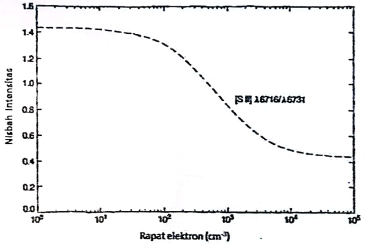
\includegraphics[scale=0.75]{sulfur.png}
        % \caption{Caption}
        % \label{fig:enter-label}
    \end{figure}

    \item Selubung PN terdiri dari gas yang terionisasi (plasma). Plasma dapat berosilasi dengan persamaan gerak berikut

    \begin{equation*}
        m_e \frac{d^2\Delta x}{dt^2} = eE
    \end{equation*}

    dengan 
    \begin{equation*}
        E=\frac{ne\Delta x}{\varepsilon_0}
    \end{equation*}
    serta $m_e$ adalah massa elektron, $e$ adalah muatan elektron, $\Delta x$ adalah perpindahan, $E$ adalah medan listrik, $n$ adalah kerapatan elektron, dan $\epsilon_0$ adalah permitivitas dengan $\varepsilon_0=8,854\times 10^{-12}$ Fm$^{-1}$. Hitunglah frekuensi plasma selubung PN tersebut. Berikan jawabanmu dalam satuan Hz.
    \item Jika bintang pusat PN merupakan bintang katai putih yang diketahui memiliki magnitudo bolometrik absolut sebesar 14, warna intrinsik $B-V = 0,30$ dan $U-V = 0,33$, serta paralaks sebesar 9 milidetik busur, maka tentukan besar ekstingsi total ($A_V$) akibat materi antarbintang dan materi di selubung PN.

    Asumsikan nisbah ekstingsi total terhadap ekstingsi selektif (\textit{total-to-selective extinction ratio}) sebesar 3,2.
    \item Jika ekstingsi antarbintang di arah PN tersebut adalah 0,7 magnitudo per kiloparsek, tentukan besar ekses warna (\textit{reddening}) yang hanya disebabkan oleh selubung PN.
\end{enumerate}


\newpage
\textit{Jawaban:}
\begin{enumerate}[a.]
    \item Kita dapat hitung panjang gelombang diam ($\lambda_0$) $H_\alpha$ menggunakan persamaan deret Balmer, terjadi ketika elektron pindah dari kulit 2 ke kulit 3 (kasus absorpsi) atau kulit 3 ke kulit 2 (kasus emisi).
    \begin{eqnarray*}
        \frac{1}{\lambda} &=& R \left( \frac{1}{2^2} - \frac{1}{3^2} \right)\\
        \lambda &=& 6562,8 \text{ \AA}
    \end{eqnarray*}
    Kecepatan radial dapat ditentukan menggunakan efek Doppler, dengan nilai panjang gelombang teramati dapat dilihat pada gambar kedua, puncaknya berada pada panjang gelombang 6566\AA.
    \begin{eqnarray*}
        \frac{\lambda - \lambda_0}{\lambda_0} &=& \frac{v_r}{c}\\
        \frac{6566 - 6562,8}{6562,8} &=& \frac{v_r}{3 \times 10^5}\\
        v_r &=& 146,28 \text{ km/s} 
    \end{eqnarray*}
    
    \item Berdasarkan potongan spektrum pada Gambar 3, kita dapat tentukan dua puncak garis Sulfur terionisasi masing-masing memiliki intensitas, 
    \begin{itemize}
        \item SII ($\lambda_0 = 6716$\AA) $\rightarrow$ $140 \times 10^{-15}$
        \item SII ($\lambda_0 = 6731$\AA) $\rightarrow$ $260 \times 10^{-15}$
        \item kontinum $\rightarrow$ $30 \times 10^{-15}$ (bagian datar jika tidak ada garis emisi, intensitasnya tidak nol)
    \end{itemize}
    Catatan: lokasi puncak garis emisi yang terlihat pada Gambar 3 sudah tidak di $\lambda_0$ karena ada redshift yang telah dihitung sebelumnya.

    Rasio intensitas dapat dihitung setelah dikurangi kontinum,
    \begin{equation*}
        \frac{140 - 30}{260-30} = \frac{110}{230} = 0,47826
    \end{equation*}
    \begin{figure}[!ht]
        \centering
        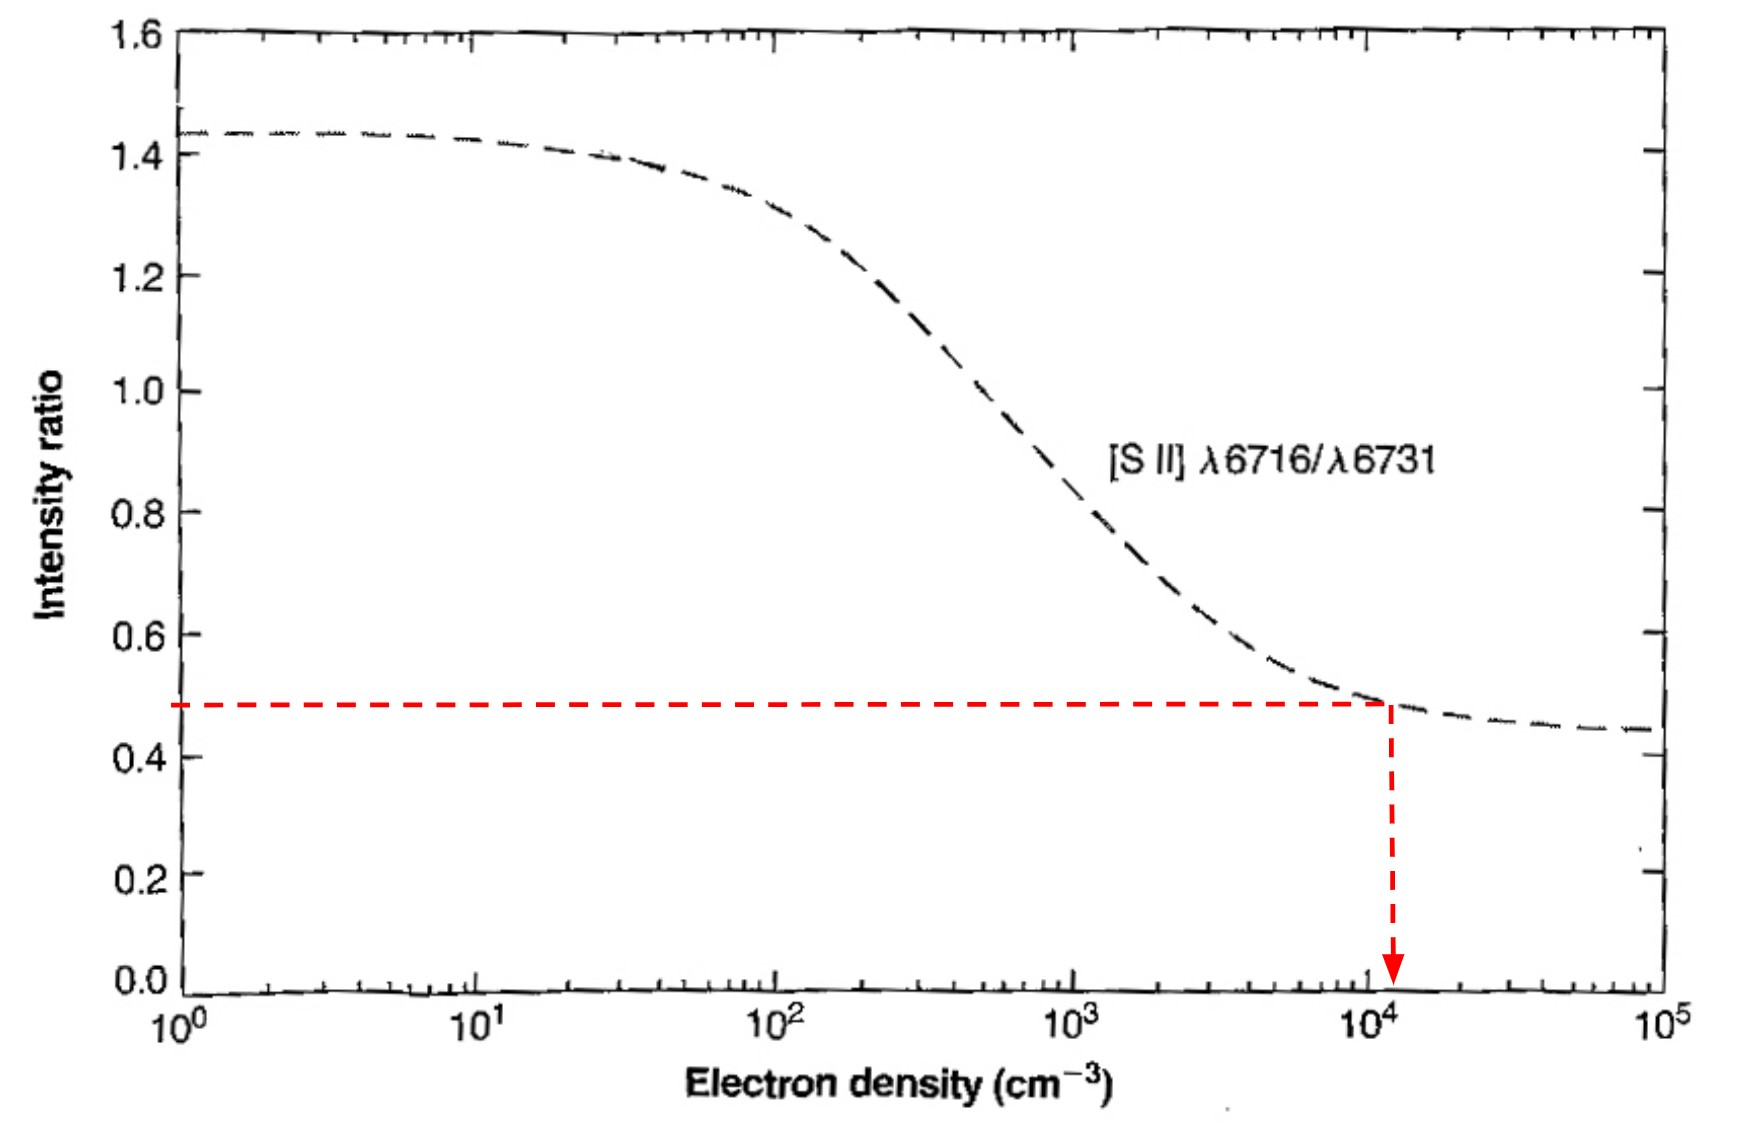
\includegraphics[width=0.6\textwidth]{sulfur_electron_density_res.jpg}
        %\caption{Caption}
        %\label{fig:enter-label}
    \end{figure}
    Menggunakan bantuan penggaris kita bisa cari titik potong antara garis horizontal $y = 0,47826$ pada plot yang diberikan untuk mencari nilai pada sumbu-$x$ (rapat elektron) yang sesuai. Kita bisa perkirakan nilai kerapatan elektron sekitar 12000 cm$^{-3}$.
    
    *Catatan: perhatikan bahwa skala yang dituliskan adalah skala logaritmik. Misalkan saja kita mengukur menggunakan penggaris, kemudian kita peroleh posisi yang diinginkan berada 2 mm di sebelah kanan $10^4$, padahal $10^4$ ke $10^5$ jaraknya 28 mm, maka nilai yang yang dimaksud adalah
    $x = 10^4 \cdot 10^{2/28} = 11787$.

    \item Frekuensi plasma
    \begin{eqnarray*}
        m_e \frac{d^2\Delta x}{dt^2} &=& e E\\
        m_e \frac{d^2\Delta x}{dt^2} &=& e \frac{ne\Delta x}{\varepsilon_0}\\
        \frac{d^2\Delta x}{dt^2} &=& \frac{n e^2}{m_e \varepsilon_0} \Delta x
    \end{eqnarray*}
    Ketika terdapat suatu persamaan diferensial di mana turunan kedua dari sebuah variabel sama dengan  variabel itu sendiri, maka salah satu solusi ``persamaan diferensial'' seperti itu yang mungkin adalah fungsi trigonometri.
    \begin{eqnarray*}
        \frac{d^2y}{dt^2} = -\omega^2 y \quad \rightarrow \text{solusinya} \quad y = A \cos{\omega t}
    \end{eqnarray*}
    Hal ini berlaku misalnya pada kasus gerak harmonik sederhana (pegas dan bandul sederhana).
    
    Melihat bentuk persamaan di atas dapat kita simpulkan frekuensi plasmanya adalah
    \begin{eqnarray*}
        \omega &=& \sqrt{\frac{n e^2}{m_e \varepsilon_0}} \\
        2 \pi f &=& \sqrt{\frac{n e^2}{m_e \varepsilon_0}} \\
        f &=& \frac{1}{2 \pi} \sqrt{\frac{n e^2}{m_e \varepsilon_0}}\\
        f &=& \frac{1}{2 \pi} \sqrt{\frac{1,2 \times 10^{-2} \cdot (1,6 \times 10^{-19})^2}{9,1 \times 10^{-31} \cdot 8,854 \times 10^{-12}}}\\
        f &=& 0,98 \approx 1 \text{ Hz}
    \end{eqnarray*}

    \item Ekstingsi total:
    \begin{eqnarray*}
        A_V &=& R_V \cdot E_{BV}\\
        A_V &=& 3,2 \cdot \left((B-V) - (B_0-V_0) \right)\\
        A_V &=& 3,2 \cdot \left((13,158-12,831) - 0,3 \right)\\
        A_V &=& 0,0864
    \end{eqnarray*}
    
    \item Jarak ke PN 
    $$d = \frac{1}{p} = \frac{1}{0,009} = 111,11 \text{ pc}$$
    
    Ekstingsi akibat materi antar bintang
    $$A_V = 0,7 \text{ mag/kpc} \cdot 0,11111 \text{ kpc} = 0,07778$$
    
    Ekses warna (\textit{reddening}) akibat selubung PN
    \begin{eqnarray*}
        E_{BV, PN} = \frac{A_{V, PN}}{R_V} = \frac{0,0864 - 0,07778}{3,2} = 0,0027
    \end{eqnarray*}
    
    
    
\end{enumerate}


\newpage 
\question Lensa gravitasi merupakan salah satu konfirmasi dari Teori Relativitas Umum (TRU) Einstein yang menjelaskan hubungan kelengkungan ruang-waktu dengan massa. Keberadaan massa di antara pengamat dan sumber cahaya akan menyebabkan kelengkungan ruang-waktu, kemudian kelengkungan tersebut yang membuat trajektori foton dari sumber cahaya latar belakang dapat difokuskan ke pengamat. Sebagai ilustrasi lihat gambar di bawah ini yang merupakan skema geometri pembentukan fenomena lensa gravitasi. $D_L$, $D_S$, dan $D_{LS}$, secara berurutan adalah jarak pengamat menuju lensa, pengamat menuju sumber, dan lensa menuju sumber. Selain itu didefinisikan sudut-sudut yang diukur dari garis pandang yaitu garis yang menghubungkan pengamat menuju pusat lensa diteruskan ke bidang sumber, $\beta$ posisi sudut sumber tak terlensakan, $\theta$ posisi sudut citra yang terbentuk, $\alpha$ sudut pembelokan, dan $\widehat{\alpha}$ adalah sudut pembelokan tereduksi.

\begin{figure}[ht!]
    \centering
    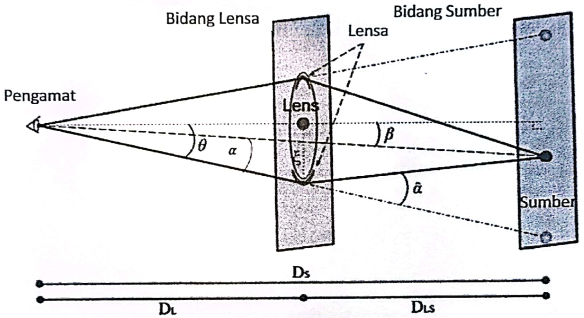
\includegraphics[scale=0.65]{lensing.png}
    % \caption{Caption}
    % \label{fig:enter-label}
\end{figure}

\begin{enumerate}[a.]
\item Jika diketahui besar sudut pembelokan tereduksi dari TRU adalah

\begin{equation*}
    \hat{\alpha} = \frac{4GM_L}{c^2\xi}
\end{equation*}

dengan $G$ konstanta gravitasi, $c$ kecepatan cahaya, $M_L$ massa objek lensa, dan $\xi$ parameter \textit{impact}, turunkan persamaan lensa gravitasi yang berupa hubungan $\beta$ sebagai fungsi dari $\theta$ (sudut yang teramati) menggunakan hubungan geometri yang diilustrasikan oleh gambar di atas!

\item Dengan  mengasumsikan bahwa sebuah bintang katai bermassa $0,5M_{\odot}$ terletak pada jarak 5,8 kpc dari pengamat di Bumi telah melensakan sebuah bintang latar belakang di sekitar pusat galaksi Bima Sakti. Hitung berapa besar radius sudut yang terbentuk ketika bintang latar belakang tepat berada di garis pandang (disebut radius Einstein)! Nyatakan dalam milidetikbusur!
\item Apakah dengan besar sudut yang diperoleh dari soal 8b akan dapat diamati menggunakan \textit{Hubble Space Telescope} (HST) dengan resolusi sudut 0,03 detikbusur?
\end{enumerate}


\newpage
\textit{Jawaban:}

Perlu diperhatikan bahwa gambar yang disediakan tidak dalam skala yang sebenarnya. Kunci pertama untuk dapat menjawab soal ini adalah menyadari bahwa sudut-sudut yang diberikan pada sketsa ($\theta, \alpha, \beta, \widehat{\alpha}$) adalah sudut yang sangat kecil, karena jarak-jarak ($D_L, D_S, D_{LS}$) yang digambarkan juga sebenarnya adalah jarak yang sangat jauh (skala kosmologi; jarak antar galaksi).

\begin{figure}[!ht]
    \centering
    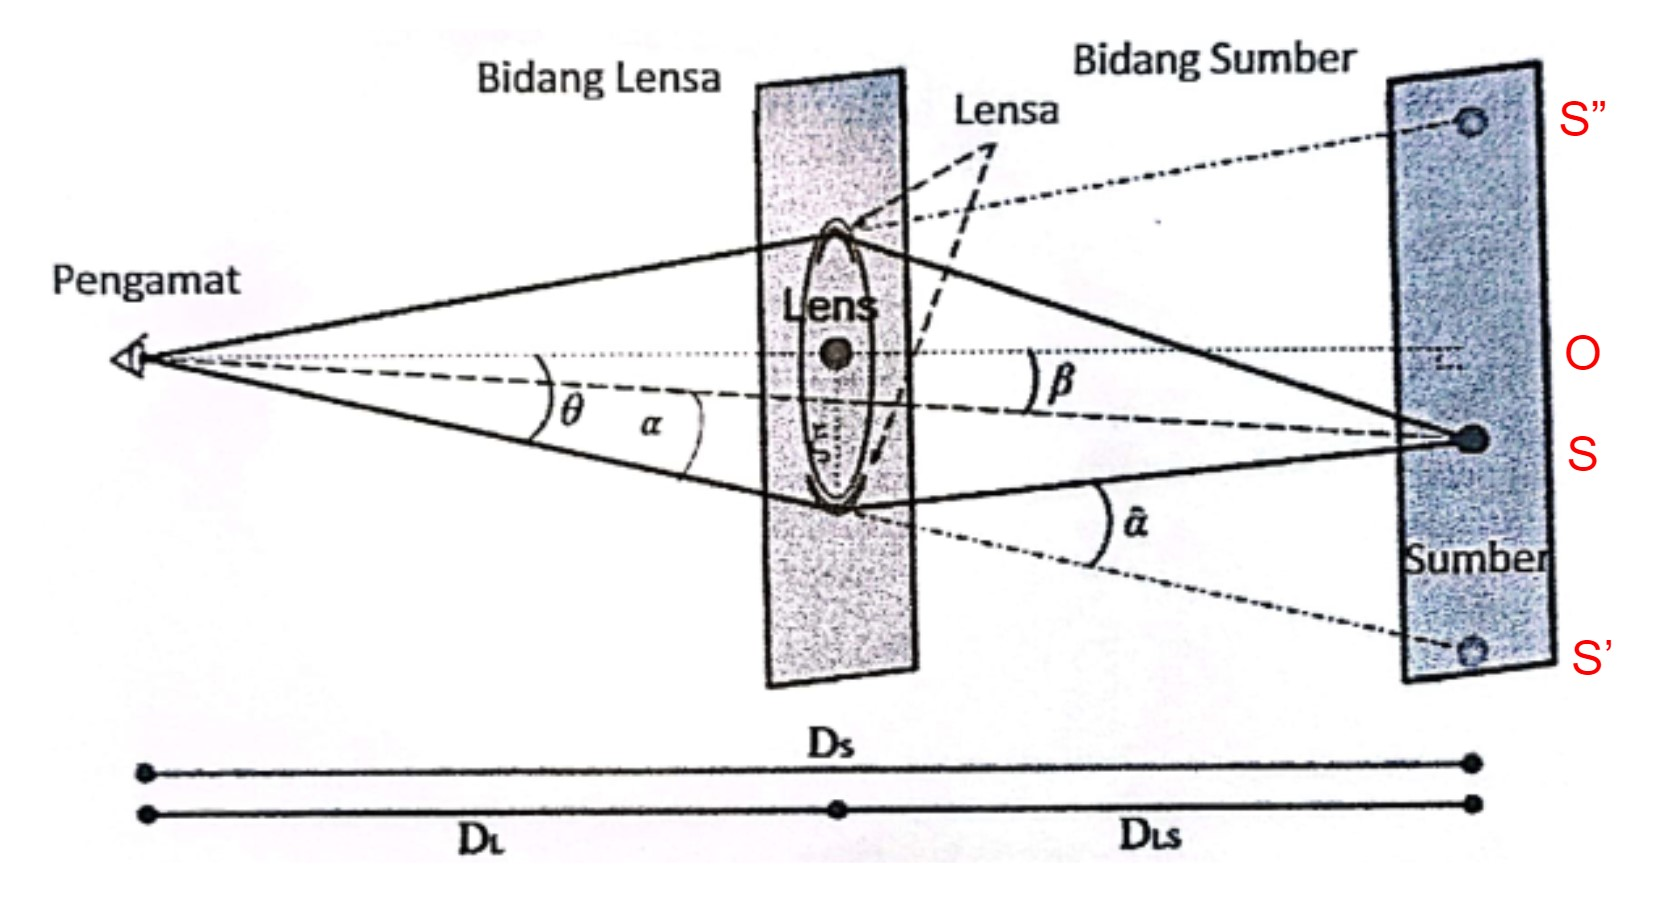
\includegraphics[width=0.7\textwidth]{lensing2.jpg}
    %\caption{Caption}
    %\label{fig:enter-label}
\end{figure}

Karena sudutnya sangat kecil, kita bisa gunakan pendekatan sudut kecil, $\sin{\theta} \approx \tan{\theta} \approx \theta_\text{rad}$, sehingga jika kita gunakan satuan sudut radian dapat kita tuliskan,
\begin{align*}
    \xi &= \theta \cdot D_L\\
    OS &= \beta \cdot D_{S}\\
    SS' &= \widehat{\alpha} \cdot D_{LS}\\
    SS' &= \alpha \cdot D_S
\end{align*}
dan kita juga memiliki hubungan,
\begin{align*}
    D_S &= D_L + D_{LS}\\
    OS' &= OS + SS'\\
    \theta &= \beta + \alpha
\end{align*}

\begin{enumerate}[a.]
    \item Kita bisa turunkan $\beta$ sebagai fungsi dari $\theta$
    \begin{eqnarray*}
        \beta &=& \theta - \alpha\\
        \beta &=& \theta - \frac{SS'}{D_S}\\
        \beta &=& \theta - \frac{\widehat{\alpha} \cdot D_{LS}}{D_S}\\
        \beta &=& \theta - \frac{D_{LS}}{D_S} \frac{4GM_L}{c^2 \xi}\\
        \beta &=& \theta - \frac{D_{LS}}{D_S} \frac{4GM_L}{c^2 \cdot \theta \cdot D_L}\\
        \beta &=& \theta - \frac{D_{LS}}{D_S \cdot D_L} \frac{4GM_L}{c^2 \theta}
    \end{eqnarray*}

    \item Kita telah turunkan $\beta(\theta)$ pada soal sebelumnya, sehingga untuk kasus sumber berada tepat di belakang lensa, $\beta = 0$, kita bisa turunkan rumus yang disebut sebagai \textit{Einstein radius}/\textit{Einstein ring},
    \begin{eqnarray*}
        \theta &=& \frac{D_{LS}}{D_S \cdot D_L} \frac{4GM_L}{c^2 \theta}\\
        \theta^2 &=& \frac{D_{LS}}{D_S \cdot D_L} \frac{4GM_L}{c^2}\\
        \theta_{E} &=& \sqrt{\frac{D_{LS}}{D_S \cdot D_L} \frac{4GM_L}{c^2}}
    \end{eqnarray*}
    Untuk lensa bermassa $M_L = 0,5 M_\odot$, jarak lensa $D_{L} = 5,8$ kpc, jarak sumber (jarak pusat galaksi) $D_S = 8$ kpc, dan jarak lensa ke sumber $D_{LS} = 8 - 5,8 = 2,2$ kpc, kita bisa hitung radius Einstein,
    \begin{eqnarray*}
        \theta_E = 2,13 \times 10^{-9} \text{ rad} = 0,44 \text{ milidetikbusur}.
    \end{eqnarray*}

    \item Radius Einstein objek tersebut (0,44 \textit{mas}) jauh lebih kecil daripada resolusi sudut HST (30 \textit{mas}), sehingga tidak dapat dipisahkan.
\end{enumerate}

\end{questions}

\vspace{3cm}
\begin{flushright}
%Hitungan lebih detail bisa di cek di \url{https://s.id/HitunganOSP2020}\\
Solusi seperti ini dapat diperoleh di \url{http://ridlow.wordpress.com}
\end{flushright}


\end{document}